% LAYOUT RULE (load-bearing): the main results table (Table 1) must render
% in or immediately after Section 6 ("The audit result") and must NEVER
% float past the references. In the v2 PDF the [t]-floated results table
% stranded itself on the last page, AFTER the bibliography
% (see audit/v2_page_images/page-15.png). This skeleton prevents that by:
%   (i)  building Table 1 as a non-floating longtable, or table[h!] guarded
%        by \FloatBarrier inside Section 6; and
%   (ii) a \FloatBarrier + \clearpage backstop before \bibliography so no
%        deferred float can ever land after the references.
%
%   pdflatex -> bibtex -> pdflatex -> pdflatex, output to build/.
%
\documentclass[11pt,a4paper]{article}

\usepackage[utf8]{inputenc}
\usepackage[T1]{fontenc}
\usepackage{lmodern}
\usepackage{amsmath,amssymb}
\usepackage{array}
\usepackage{booktabs}
\usepackage{longtable}
\usepackage{graphicx}
\usepackage{xcolor}
\usepackage[margin=1in]{geometry}
\usepackage[hidelinks]{hyperref}
\usepackage{caption}
\usepackage{microtype}
\usepackage{placeins}
\setlength{\emergencystretch}{3em}

\title{widom-atlas: Auditing Widom-Insertion Recipes for Zero-Coverage Adsorption}
\author{Onur Alexander William Aydogan\\
Waynestark Enterprises Limited}
\date{}

\begin{document}

\maketitle

\begin{abstract}
Widom insertion gives well-defined zero-coverage adsorption observables only after the host structure, atom typing, force field, gas model, mixing rule, electrostatics, backend, sampling protocol, and reference observable have been specified. In materials screening, the resulting Henry constant \(K_H\) and zero-coverage isosteric heat \(Q_{st}\) are often treated as properties of the material, but they are in fact outputs of this complete recipe. We present widom-atlas, a governed validation harness that locks each recipe as a branch, compares the resulting observable with one stated experimental reference, and classifies the outcome as a strict pass, a physical-accuracy pass, a force-field disagreement, a reference-observable mismatch, a structural blocker, or an ensemble/method mismatch. In v0.4, presented as method-plus-audited-examples rather than a fifteen-branch certification, two of fifteen verdict-affecting branches pass the strict criterion --- an all-silica MFI + Ar positive control and a UiO-66 + CO\(_2\) branch under genuine Universal Force Field (UFF) --- and five of fifteen pass the broader Tier-B physical-accuracy criterion (those two, plus HKUST-1 + CO\(_2\) under genuine UFF, the Si-CHA + CO\(_2\) Bai 2013 control, and the UiO-66 explicit-hydrogen Maia 2023 variant). Two of those passes (HKUST-1 and UiO-66) were recovered only after the audit caught a generator silently substituting guest and zeolite parameters under a false ``UFF'' label on the framework atoms; corrected to genuine UFF, the linker dispersion compensates the weak open-metal site and both MOFs reproduce experiment. The remaining branches expose force-field transferability limits at the Mg-MOF-74 open metal site, reference-observable mismatches, missing cationic-zeolite structures and cation models, and a Na-Rho trapdoor ensemble mismatch. A subsequent extension retargets the harness onto CuspAI's kUPS engine and the machine-learned potential it ships: it provides, to our knowledge and based on public-source searches conducted on 15 June 2026, the first published independent cross-engine validation of the Widom estimator shipped in kUPS --- the \texttt{kups.mcmc.widom} module specifically, as distinct from standalone Widom packages and from machine-learned-potential adsorption benchmarks such as ODAC25~\cite{ODAC25}; that same cross-engine audit found the originally-locked MFI + Ar positive control had \emph{double-counted silicon}: it still landed inside the strict band, but only as a fortuitous cancellation of four compounding errors --- a coincidence, not a coherent result --- and rebuilding it clean on the calibration (Olson) geometry reproduces the corrected reference \(K_H = 0.200\) exactly and cross-engine (the project's native estimator 0.200, RASPA3 0.199) --- with the isosteric heat reproduced to 0.01--0.22 kJ/mol on two locked controls, the dominant \(K_H\) discrepancies traced to named conventions and one normalization-flavoured residual on the electrostatic control flagged open, and a governed out-of-distribution demonstration on machine-learned potentials that discriminates over-binding from missing-dispersion failure, screen-passes a dispersion-corrected route for the latter, and withholds a verdict on a foundation model used outside its training domain. widom-atlas is therefore not scientifically validated as a general predictive adsorption tool. It is a reproducible way to decide whether a particular Widom adsorption number is a trustworthy zero-coverage observable or merely the output of an untested recipe.
\end{abstract}

% ====================== MAIN TEXT (Sections 1--9) ======================
% Section 1 --- The problem
% the only applied change is the approved citation-key fix
% Dunne1996 -> Dunne1996Langmuir.
\section{The problem}\label{sec:problem}

A materials-discovery calculation often begins with a simple request: rank porous crystals by how strongly they adsorb a gas at low pressure. For a zeolite or a metal-organic framework, the desired quantities are usually the Henry constant, \(K_H\), and the zero-coverage isosteric heat, \(Q_{st}\). They are attractive screening targets because they are cheaper than full isotherms and because they seem to measure the first contact between a guest molecule and a host framework.

Widom insertion appears to supply exactly these quantities. In its simplest form, the method inserts a ghost molecule into a host, evaluates the host-guest energy, and averages the corresponding Boltzmann weight. In the dilute limit this is a well-defined statistical-mechanical estimator \cite{FrenkelSmit2002}. The apparent simplicity is the danger. The estimator may be exact for a specified model, but the prediction is not exact for the material unless the model is the right one.

A Widom adsorption number is therefore not a freestanding fact about a crystal. It is the result of a recipe. The recipe includes the crystallographic structure, atom typing, force field, gas model, cross-pair mixing rule, electrostatics, simulation backend, sampling rule, and experimental reference observable. Changing any one of these ingredients changes the scientific meaning of the number. A calculation can be reproducible and still be wrong if the structure is the wrong state, the force field binds the guest incorrectly, or the reference value was extracted from a different thermodynamic observable.

This distinction matters for materials discovery. A screening workflow can use a wrong adsorption score just as easily as a correct one. If the score is treated as a property of the material rather than as the output of a recipe, then a model may be optimised against a hidden mixture of structure error, force-field error, reference mismatch, and method mismatch. The result is not merely numerical noise. It is a false target.

The purpose of widom-atlas is to make that hidden recipe visible and testable. Each branch fixes one complete recipe before it is run. The branch then compares the resulting \(K_H\) and \(Q_{st}\), when those observables are defined, to one stated experimental reference. The outcome is not collapsed into a single success score. It is classified as a strict pass, a Tier-B physical-accuracy pass, a force-field disagreement, a reference-observable mismatch, a structural blocker, or an ensemble/method mismatch.

The distinction between these classes is essential. If a non-polarisable force field over-binds carbon dioxide at an open metal site, the answer is not to call Widom insertion wrong. If a cationic zeolite is represented by a pure-silica framework, the calculation is testing the wrong material. If a trapdoor zeolite opens during adsorption but the simulation samples only a rigid closed structure, the calculation and experiment are not evaluating the same partition function. These are different scientific failures, and treating all of them as ordinary pass/fail errors hides the physics.

Version 0.4 is therefore not presented as a general predictive adsorption tool, and the classical matrix is reported as method-plus-audited-examples rather than a fifteen-branch certification. Its locked result is narrow: two of fifteen verdict-affecting branches pass the strict criterion --- an all-silica MFI + Ar positive control \cite{Talu2001,Dunne1996Langmuir} and a UiO-66 + CO\(_2\) branch under genuine Universal Force Field (UFF) --- and five of fifteen pass the broader Tier-B physical-accuracy criterion, adding HKUST-1 + CO\(_2\) under genuine UFF, the Si-CHA + CO\(_2\) Bai 2013 branch compared with the Maghsoudi 2013 reference \cite{Bai2013JPCC,Maghsoudi2013Adsorption}, and the UiO-66 + CO\(_2\) Maia 2023 explicit-hydrogen variant \cite{Maia2023Crystals,Cmarik2012Langmuir}. The HKUST-1 and UiO-66 UFF passes were recovered only after the audit corrected a generator that had silently substituted guest and zeolite parameters under a false ``UFF'' framework label (Section~\ref{sec:result}). The Na-Rho + CO\(_2\) scalar branch is not counted as a scalar pass or fail because rigid closed-state Widom and open-state trapdoor adsorption are different observables \cite{Lozinska2012JACS,Verma2017ChemMater}.

The claim of this paper is consequently modest but useful. widom-atlas does not prove that Widom insertion with standard force fields is generally predictive. It proves that a Widom prediction can be made auditable branch by branch. In clean cases the recipe can reproduce experiment. In difficult cases the harness identifies whether the failure belongs to the force field, the reference, the structure, or the ensemble. That is the scientific object of the paper: not a universal adsorption calculator, but a governed way to decide whether a given Widom number should be trusted.

\textbf{Reader note on internal labels.} Codes such as \texttt{6c}, \texttt{3a}, \texttt{2a}, \texttt{4c}, and \texttt{3b\_EHq} are internal locked-recipe identifiers, not chemistry notation: each denotes one complete Widom-insertion recipe (a specific host structure, guest model, force field, charge model, mixing rule, electrostatics convention, simulation backend, sampling protocol, and reference observable). The ones used repeatedly below are branch 6c, the all-silica MFI + Ar positive control; branch 3a, UiO-66 + CO\(_2\) under genuine UFF; branch 2a, HKUST-1 + CO\(_2\) under genuine UFF; branch 4c, the Si-CHA + CO\(_2\) Bai 2013 control; and branch 3b\_EHq, the UiO-66 + CO\(_2\) Maia 2023 explicit-hydrogen, charged variant. ``Tier-A strict'' (\(|\Delta\log_{10}K_H|\le0.10\) and \(|\Delta Q_{st}|\le2.0\ \mathrm{kJ\,mol^{-1}}\)) and ``Tier-B physical-accuracy'' are the two pass bands defined in Section~\ref{sec:controls}. ``Native'' denotes this project's own independent Python Widom estimator --- a specific implementation, not a generic term --- used alongside the external Monte Carlo engines RASPA3 and RASPA2. The version labels are internal repository milestones: v0.4 is the locked classical audit matrix, v0.4.2 is the corrected rebuild and provenance layer for the audited examples, v0.5 is non-load-bearing consolidation or extension material, and v0.6 is the kUPS and MLIP governance companion (Section~\ref{sec:v06}).

% Section 2 --- The observable
% except the final paragraph, which the author revised before insertion to
% align with the four-class taxonomy ("three" -> "four broad reasons").
\section{The observable}\label{sec:observable}

The word ``adsorption'' hides several different thermodynamic questions. One may ask how much gas a material holds at one bar, how an isotherm bends as sites fill, how quickly a molecule enters a pore, or where the first molecule sits at infinite dilution. Widom insertion answers only the last of these questions. It gives the zero-coverage limit of adsorption for a specified rigid host and a specified host-guest energy model.

The calculation can be described before writing any equation. A guest molecule is placed into the empty framework without allowing it to perturb the framework or other guests. This test molecule is then moved through many random positions and orientations. At each insertion the interaction energy \(U\) between the test molecule and the host is evaluated. Attractive insertions contribute large Boltzmann weights, repulsive insertions contribute small weights, and severe overlaps contribute essentially nothing.

The Henry constant follows from this average. In the dilute limit, loading is proportional to pressure, and the proportionality constant is \(K_H\). Widom insertion estimates that proportionality by averaging \(\exp(-\beta U)\), with \(\beta = 1/k_B T\). A second weighted average gives the mean energy of those insertions that actually contribute to adsorption. With the usual ideal-gas thermal term, this gives the zero-coverage isosteric heat \(Q_{st}\) \cite{FrenkelSmit2002}.

For a guest in a rigid host at temperature \(T\), the estimators used in widom-atlas are

\[
K_H =
\frac{V}{M k_B T N_A}
\left\langle \exp(-\beta U)\right\rangle,
\]

and

\[
Q_{st}
=
-\frac{
\left\langle U \exp(-\beta U)\right\rangle
}{
\left\langle \exp(-\beta U)\right\rangle
}
+ RT,
\]

where \(V\) is the simulation-cell volume, \(M\) is the simulation-cell mass, \(N_A\) is Avogadro's constant, and the brackets denote the insertion average over position and orientation. The first expression is reported in \(\mathrm{mol\,kg^{-1}\,bar^{-1}}\). The second is reported in \(\mathrm{kJ\,mol^{-1}}\). Unit conversion is therefore part of the recipe, not a formatting detail.

These equations are exact only after the model has been specified. The word ``model'' includes the crystallographic coordinates, atom typing, partial charges, non-bonded parameters, mixing rule, electrostatics, cutoff, tail correction, gas geometry, and backend implementation. If those ingredients are held fixed, the insertion average has a clear statistical meaning. If they are not held fixed, two calculations called ``Widom insertion'' may be different experiments.

This is why widom-atlas treats an input recipe as a scientific object. A branch is not defined by the host name alone. ``MFI + methane'' is not a unique calculation. It becomes a calculation only after one states the MFI structure, the methane model, the framework force field, the mixing rule, the electrostatics convention, the cutoff, the backend, the temperature, and the reference observable. The same physical material can therefore appear in several branches if those recipes differ.

The estimator also has physical limits. It samples a rigid host. It does not relax a framework, move an extra-framework cation to open a window, or change the protonation or defect state of a material. It samples zero coverage. It does not reproduce a finite-loading isotherm unless that isotherm has first been extrapolated to the Henry regime. It samples the chosen potential-energy surface. It cannot repair a force field that gives the wrong binding energy at an open metal site.

These limits are not defects of Widom insertion. They are the conditions under which the observable is defined. A correct Widom calculation can therefore disagree with experiment for four broad reasons: the energy model may be wrong, the reference value may not be the same zero-coverage observable, the structure may not be the experimental material, or the sampled ensemble may not be the ensemble accessed in the experiment. The remainder of the paper uses this distinction to interpret the v0.4 branches.

% Section 3 --- The recipe
% only normalisation is LaTeX quote glyphs (smart-quotes -> ``...''), which
% render identically. No wording changed.
\section{The recipe}\label{sec:recipe}

A recipe is the complete set of choices that turns the formal Widom estimator into a particular calculation. In widom-atlas, a recipe is not an informal note in a methods paragraph. It is the object that is locked, executed, compared, and judged. This is the central design choice of the harness (Figure~\ref{fig:recipe}).

\begin{figure}[tbp]
\centering
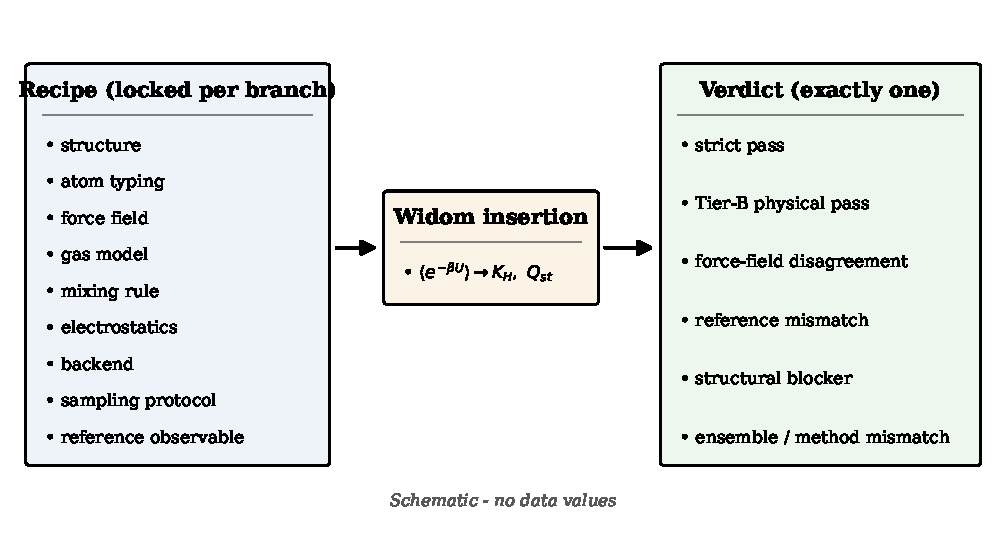
\includegraphics[width=0.92\textwidth]{figures/fig1_recipe_schematic.pdf}
\caption{A Widom adsorption number is the output of a complete recipe. The locked ingredients (left) feed Widom insertion (centre), whose zero-coverage \(K_H\) and \(Q_{st}\) are classified into exactly one of six verdicts (right). This figure is schematic and carries no numerical data.}
\label{fig:recipe}
\end{figure}

The first ingredient is the host structure. A zeolite topology name or a MOF name is not enough. The calculation needs the actual atomic coordinates, cell parameters, atom labels, and framework state. An all-silica CHA structure and a cationic chabazite are not the same material for carbon dioxide adsorption. A closed Na-Rho structure and an open Na-Rho adsorption state are not the same ensemble. A defective UiO-66 sample and an ideal UiO-66 crystal are not guaranteed to have the same low-pressure adsorption thermodynamics.

The second ingredient is the energy model. The force field defines how the guest sees the host. For a Lennard-Jones branch this means \(\epsilon\), \(\sigma\), charges, and the cross-pair rule. For Buckingham or exponential-attraction branches it means a different functional form and a different set of parameters. The gas model also matters: carbon dioxide can be represented by different charge distributions and Lennard-Jones sites, while methane can be a united-atom model or a more detailed model. These choices change \(U\), and therefore change both \(K_H\) and \(Q_{st}\).

The third ingredient is the long-range and truncation convention. Electrostatics may be absent, Ewald-summed, or represented differently by different engines. A Lennard-Jones cutoff may be used with or without an analytical tail correction. These are not cosmetic simulation settings. In the Si-CHA + CO\(_2\) branch, the analytical tail correction is part of the successful recipe because it shifts the Henry constant from the edge of the strict band into its interior.

The fourth ingredient is the backend. A backend is not merely a calculator button. It is the implementation that evaluates \(U\). RASPA3, RASPA2, the native widom-atlas evaluator, and the ASE-wrapper route can represent different subsets of force-field forms. A branch must therefore state which backend was used and why that backend is capable of representing the recipe.

The fifth ingredient is the reference observable. A number from the literature is not automatically the number that Widom insertion predicts. The reference may be a Henry slope, a Toth or Langmuir fit, a van't Hoff heat, a calorimetric heat, a finite-loading value, a breakthrough quantity, a site distance, or a kinetic parameter. widom-atlas treats these as different observables. It compares \(K_H\) and \(Q_{st}\) only when the reference can be defended as the same zero-coverage thermodynamic quantity.

This recipe view explains why branches, not materials, are the units of the atlas. MFI + CH\(_4\), MFI + Ar, and MFI + Kr share a framework family, but they are different recipes because the gas model, cross-pair parameters, reference values, and sometimes validation purpose differ. UiO-66 + CO\(_2\) also appears in more than one recipe because framework charges, explicit hydrogens, and literature reference choices change the calculation. The atlas must preserve those distinctions rather than average them away.

The recipe view also explains why a blocked branch is not a failed computation. If a cationic-zeolite reference has a clean Henry constant but the corresponding cation-containing CIF and cation force field are not locked, the scientific state is not ``FAIL''; it is ``not yet a defined calculation.'' If Na-Rho adsorption requires a gate-open framework state that rigid closed-state Widom does not sample, the scientific state is not ``bad parameter choice''; it is an ensemble mismatch. These labels prevent the atlas from manufacturing certainty where the recipe is incomplete.

For this reason, the case matrix is the scientific ledger of widom-atlas. It records the structure, atom typing, force-field form, gas model, mixing rule, electrostatics, backend, sampling protocol, reference observable, threshold, and verdict class for each branch. Once locked, the branch can be run, checked, and re-run. If the number changes without a recipe change, that is an implementation problem. If the number is stable but disagrees with the reference, the disagreement belongs to the recipe or to the reference, not to the Widom estimator in isolation.

% Section 4 --- The harness
% only normalisation is the required LaTeX underscore escape in the literal
% branch id 3b_EHq -> 3b\_EHq (renders identically). No wording changed.
\section{The harness}\label{sec:harness}

The practical role of widom-atlas is to turn the recipe described above into something that can be inspected and re-run. A recipe that lives only in prose is too easy to change without noticing. A force-field file may be edited, a framework atom label may be relabelled, a backend may change its defaults, or a reference value may be copied with a different interpretation. The harness is designed to prevent those changes from being silent.

The central object is the case matrix. It is a machine-readable ledger in which every verdict-affecting branch records its structure, atom typing, force field, gas model, mixing rule, electrostatics, backend, sampling protocol, reference observable, threshold, and verdict class. The v0.4 matrix is pinned by a SHA-256 digest,

\[
\mathrm{CASE\_MATRIX\_SHA256}
=
\texttt{b0571780\ldots a085664}.
\]

The full digest is recorded in the reproducibility appendix. The point of the hash is simple: if the recipe changes, the identity of the calculation changes. The loader therefore checks the matrix before execution, so a result cannot be read as a v0.4 result after the locked input has changed.

A branch is then executed by the backend capable of representing its energy model. Ordinary Lennard-Jones and Ewald branches can be run through RASPA3. Buckingham branches that need the older parametrisation path can be run through RASPA2. Branches whose functional forms are not expressible in the tested RASPA path are run with the native widom-atlas evaluator. An ASE-calculator route is kept for interoperability and independent driver checks. The backend is recorded because it is part of the calculation, not an implementation footnote.

The harness also separates numerical execution from scientific judgement. First, the branch is run and the raw \(K_H\) and \(Q_{st}\) estimates are produced with their sampling uncertainty. Second, the estimates are compared with the specified reference observable. Third, the comparison is assigned a scientific interpretation. This prevents a single numerical difference from being treated as self-explanatory. The same deviation could indicate a transferable-force-field problem, a mismatched reference, a wrong structure, or a method mismatch.

Two acceptance bands are used. The strict band is a regression and reproducibility gate: \(\pm 0.10\) in \(\Delta \log_{10} K_H\) and \(\pm 2.0\ \mathrm{kJ\,mol^{-1}}\) in \(\Delta Q_{st}\). It is deliberately tight, and passing it means that the locked recipe reproduces the chosen reference within that strict tolerance. The physical-accuracy band is broader and system-specific. It is used when the literature itself shows enough spread that a stricter numerical gate would confuse physical scatter with implementation error.

This distinction is important for the v0.4 disposition. The strict result is two passes out of fifteen verdict-affecting branches: 6c, the all-silica MFI + Ar positive control, and 3a, the UiO-66 + CO\(_2\) branch under genuine UFF (recovered after the audit corrected a mislabelled framework force field; Section~\ref{sec:result}). The physical-accuracy result is five passes out of fifteen: 6c, 3a, 2a (HKUST-1 + CO\(_2\) under genuine UFF), 4c (Si-CHA + CO\(_2\) under the Bai 2013 TraPPE-zeo recipe), and 3b\_EHq (UiO-66 + CO\(_2\) under the explicit-hydrogen, Yang-charge Maia 2023 variant). Branches 2a, 4c, and 3b\_EHq do not pass the strict gate but lie inside the Tier-B band defined for their systems.

The verdict labels are therefore not decorations added after the calculation. They are part of the scientific record. A strict pass means the branch passes both axes of the strict comparison. A Tier-B physical pass means the branch does not satisfy the strict regression gate but is still within the system-specific physical-accuracy band. A force-field disagreement means that the estimator and implementation may be sound, but the energy model does not reproduce the reference. A reference-observable mismatch means the calculation and the literature number are not the same thermodynamic quantity. A structural blocker means that the simulated structure is missing, incomplete, or not the experimental material. An ensemble or method mismatch means that the calculation samples a different configuration space from the experiment.

The harness is conservative by design. It does not rescue a branch by changing the recipe after seeing the result. It does not average incompatible references into a convenient target. It does not treat an unexecutable branch as a hidden success. It records the reason a branch passes, fails, or cannot yet be judged. That conservatism is why the current result is scientifically useful even though the pass count is small.

This design also makes the work falsifiable. A future reader can inspect the branch, reproduce the recipe, run the backend, and compare the output with the same reference. If the result changes, the change must be traced to the code, the dependency stack, the backend, or the locked inputs. If the result does not change but still disagrees with experiment, the disagreement belongs to the scientific model or the reference observable. The harness does not remove judgement from adsorption validation; it makes the judgement auditable.

% Section 5 --- The controls
% only normalisation is LaTeX quote glyphs in the final paragraph
% (smart-quotes -> ``...''), which render identically. No wording changed.
% All 6c/4c numbers and the V1-V4 percentages were verified against the lock.
\section{The controls}\label{sec:controls}

Before a validation harness is allowed to blame a force field, a structure, or a reference, it must first show that its own machinery is not the cause of the disagreement. The controls in v0.4 answer that narrower question. They do not prove that Widom insertion is generally predictive. They prove that, for recipes whose ingredients are compatible with the tested backends and references, the harness can reproduce known zero-coverage observables.

The first control is backend agreement. When two independent implementations can represent the same recipe, they should return the same adsorption observable within the expected sampling error. The native Lennard-Jones evaluator agrees with RASPA3 to within one percent on the all-silica MFI + Ar and MFI + CH\(_4\) recipes. On the Si-CHA + CO\(_2\) charged-framework control (4c) the native Ewald estimator and RASPA3 agree to \(\sim\!9\%\) on \(K_H\) and \(\sim\!1\%\) on \(Q_{st}\). On HKUST-1, by contrast, the native charged-Ewald path shows a large empirical discrepancy against RASPA3 --- about a factor of four on the identical recipe. A suspected non-orthogonal minimum-image explanation was tested after the audit: at the actual supercells and cutoffs of the published runs, a brute-force image check found no within-cutoff mis-imaged pairs for HKUST-1, Si-CHA, or MFI, so the root cause is not established. We therefore treat native charged-MOF results as non-verdict-supporting: the MOF branches are reported from RASPA3 (2a, 3a) or RASPA2 (1a), or presented as audited examples with this limitation stated (1b, 1c, 1d, 2b, 3b). The 4c result is retained because it is directly cross-engine checked, not because of any orthogonality assumption. The Mg-MOF-74 + CO\(_2\) Buckingham recipe was run on RASPA2; the native Buckingham path is not independently cross-validated on this MOF. No headline result depends on the native charged-MOF path. These tests are not the scientific result of the paper, but they are the guardrail that makes later disagreement with experiment interpretable.

The second control is deliberately simple. Branch 6c is all-silica MFI + Ar. It has no host charges, no open metal site, no framework gate, and no flexible cation sublattice. The calculation uses a rigid all-silica MFI framework on Talu-Myers' calibration geometry (Olson 1981), an argon probe under Talu's single-source oxygen-only potential, and two independent estimators --- a native Lennard-Jones evaluator and RASPA3 --- at a converged cutoff with analytical tail correction. (Branch 6c was rebuilt in v0.4.1: the originally-locked recipe silently double-counted silicon and was scored against a mis-derived reference; the corrected single-source recipe, and the four-error cancellation it replaces, are documented in Section~\ref{sec:v06}, Finding~F1.) This is close to the cleanest adsorption problem in the atlas: if this branch failed, the harness would have no right to interpret more difficult failures.

It does not fail. Against the Talu-Myers and Dunne references, branch 6c gives

\[
K_H = 0.200 \pm 0.003\ \mathrm{mol\,kg^{-1}\,bar^{-1}},
\qquad
Q_{st} = 14.97\ \mathrm{kJ\,mol^{-1}},
\]

with

\[
\Delta \log_{10} K_H = 0.000,
\qquad
\Delta Q_{st} = -0.73\ \mathrm{kJ\,mol^{-1}}.
\]

Both deviations are inside the strict band --- the Henry constant matches the corrected reference (\(0.200\ \mathrm{mol\,kg^{-1}\,bar^{-1}}\)) to within sampling error, and the heat is within \(0.73\ \mathrm{kJ\,mol^{-1}}\) of the calorimetric reference (\(Q_{st} = 15.7\ \mathrm{kJ\,mol^{-1}}\)) --- so 6c is a Tier-A strict pass, cross-confirmed by the native estimator and RASPA3 (parity \(0.5\%\)) \cite{Talu2001,Dunne1996Langmuir}. The result is important not because argon in silicalite is technologically surprising, but because it shows that the pipeline can reproduce a clean reference when the physical problem is simple.

The third control is less trivial. Branch 4c tests all-silica Si-CHA + CO\(_2\), using the Bai 2013 TraPPE-zeo framework parameters, TraPPE CO\(_2\), native Ewald electrostatics, and an analytical Lennard-Jones tail correction. The branch is run over three seeds of 60,000 insertions and compared with the Maghsoudi 2013 zero-coverage reference. This case is still an all-silica zeolite, but it includes electrostatics, a multi-site quadrupolar guest model, and a tail correction that materially affects the Henry constant.

Branch 4c is a cross-engine-audited charged control whose strict-versus-Tier-B verdict is itself engine-dependent. On the native estimator it gives

\[
K_H = 2.22 \pm 0.14\ \mathrm{mol\,kg^{-1}\,bar^{-1}},
\qquad
Q_{st} = 22.99 \pm 0.33\ \mathrm{kJ\,mol^{-1}},
\]

with \(\Delta \log_{10} K_H = -0.039\) and \(\Delta Q_{st} = +1.99\ \mathrm{kJ\,mol^{-1}}\) --- just inside the strict band. A faithful RASPA3 cross-check of the identical recipe (TraPPE-CO\(_2\), Ewald, \(14\)~\AA{} + tail) gives \(K_H = 2.03\) and \(Q_{st} = 23.24\ \mathrm{kJ\,mol^{-1}}\), i.e.\ \(\Delta \log_{10} K_H = -0.079\) and \(\Delta Q_{st} = +2.24\ \mathrm{kJ\,mol^{-1}}\) --- just outside. The reference values are \(K_H = 2.43\ \mathrm{mol\,kg^{-1}\,bar^{-1}}\) and \(Q_{st} = 21.0\ \mathrm{kJ\,mol^{-1}}\) \cite{Bai2013JPCC,Maghsoudi2013Adsorption}; both engines sit inside the experimental window \([1.9, 3.0]\) and agree to \(\sim\!9\%\) on \(K_H\) and \(\sim\!1\%\) on \(Q_{st}\). But the \(Q_{st}\) deviation straddles the \(\pm 2.0\) boundary (native \(+1.99\), inside; RASPA3 \(+2.24\), outside), so the same recipe is nominally strict on one engine and Tier-B on the other. We therefore report 4c as a Tier-B cross-engine-audited control, and note this as a worked example, on a charged system, of the verdict fragility this harness exists to expose. The tail correction is part of the recipe: it shifts the native Henry constant from \(1.98\) to \(2.22\ \mathrm{mol\,kg^{-1}\,bar^{-1}}\), moving \(\Delta \log_{10}K_H\) from \(-0.089\) to \(-0.039\), rather than being a hidden numerical default.

These controls define the safe interpretation of the rest of the paper. They show that widom-atlas can reproduce experiment --- with two independent engines agreeing on it --- when the host structure is well defined, the force field is appropriate for the chemistry, and the reference is compatible with the zero-coverage observable. They do not show that every subsequent branch ought to pass. On the contrary, they make later failures more informative. Once the clean controls pass, a persistent failure in an open-metal-site MOF, a cationic zeolite, or a trapdoor framework is no longer plausibly dismissed as merely a broken Widom implementation.

The controls therefore narrow the question. The remaining branches ask not ``does the code run?'' but ``does this locked recipe correspond to the experimental observable it is being asked to reproduce?'' That is the question the audit answers.

% Section 6 --- The audit result
% author had already escaped 3b\_EHq; no smart-quotes present). Table 1 is
% built separately at tables/table1_branch_disposition.tex (non-floating
% longtable) and \input here, in-section, immediately after the
% label-definition paragraph. Every number was verified against the lock and
% the v04 verdict JSONs.
\section{The audit result}\label{sec:result}

The v0.4 audit is presented as method-plus-audited-examples, not a fifteen-branch certification: it does not validate Widom adsorption prediction in general, but it establishes a small set of clean controls and audit-corrected examples within their stated bands and documents the defects the audit caught. The strict result is two passes out of fifteen verdict-affecting branches: the clean MFI + Ar control, branch 6c, and the UiO-66 + CO\(_2\) branch under genuine UFF, branch 3a (Figure~\ref{fig:strict}). The Tier-B physical-accuracy result is five passes out of fifteen: 6c, 3a, the HKUST-1 + CO\(_2\) branch 2a (genuine UFF), the Si-CHA + CO\(_2\) Bai 2013 branch 4c, and the UiO-66 + CO\(_2\) explicit-hydrogen, Yang-charge branch 3b\_EHq (Figure~\ref{fig:disposition}).

Table~\ref{tab:branch-disposition} gives the branch-level disposition. It should be read as a map of causes, not as a leaderboard. A strict pass means that both \(K_H\) and \(Q_{st}\) lie inside the tight regression band. A Tier-B pass means that the branch fails the strict gate but remains inside the broader physical-accuracy band justified for that system. A force-field disagreement means that the energy model does not reproduce the selected reference. A reference-observable mismatch means that the literature number and the Widom zero-coverage quantity are not the same observable. A structural blocker means that the simulated structure is missing, incomplete, or not the experimental material. An ensemble or method mismatch means that the calculation samples a different configuration space from the experiment.

% Table 1 --- branch-level disposition. Built 2026-06-09.
% tables/table1_branch_disposition.source.md. Non-headline deltas were
% re-read directly from evidence/v04_two_tier/verdicts/*.json (and 6e from
% evidence/v04_6e_bai_2013/verdicts/6e.json); 6c/4c/3b_EHq from the lock.
% NON-FLOATING longtable. Do not convert to table[t]. Label: tab:branch-disposition.
{\scriptsize
\setlength{\tabcolsep}{3pt}
\renewcommand{\arraystretch}{1.25}
\begin{longtable}{@{}>{\raggedright\arraybackslash}p{0.072\textwidth}>{\raggedright\arraybackslash}p{0.105\textwidth}>{\raggedright\arraybackslash}p{0.225\textwidth}r r >{\raggedright\arraybackslash}p{0.10\textwidth}>{\raggedright\arraybackslash}p{0.165\textwidth}@{}}
\caption{Branch-level disposition of the v0.4 audit. The headline strict-pass
denominator is fifteen verdict-affecting scalar branches. The UiO-66 3b family
is shown in three force-field variants for scientific transparency but is
counted according to the locked v0.4 disposition; branch 5b is shown as
method-blocked and is not scored as a scalar $K_H$/$Q_{st}$ pass or fail. The
Tier-A strict passes are 6c and 3a. The Tier-B physical-accuracy passes are 6c,
3a, 2a, 4c, and 3b\_EHq. Branches 2a and 3a are the v0.4.2 genuine-UFF rebuild
(superseded as-locked deviations in parentheses); 4c is reported on RASPA3 as
Tier-B, its strict label being engine-marginal. Branch identifiers are internal
locked-recipe labels, retained only to keep the table traceable to the repository
and its evidence JSON; for example 6c = all-silica MFI + Ar, 3a = UiO-66 +
CO\textsubscript{2} (genuine UFF), 2a = HKUST-1 + CO\textsubscript{2} (genuine
UFF), 4c = Si-CHA + CO\textsubscript{2} (Bai 2013 control), and 3b\_EHq = UiO-66 +
CO\textsubscript{2} (Maia 2023 explicit-hydrogen, charged).}\label{tab:branch-disposition}\\
\toprule
Br. & System & Recipe (structure / force field / gas) & $\Delta\log_{10}K_H$ & $\Delta Q_{st}$ & Class & Reason \\
\midrule
\endfirsthead
\multicolumn{7}{@{}l}{\footnotesize\emph{Table~\ref{tab:branch-disposition}, continued}}\\
\toprule
Br. & System & Recipe (structure / force field / gas) & $\Delta\log_{10}K_H$ & $\Delta Q_{st}$ & Class & Reason \\
\midrule
\endhead
\midrule
\multicolumn{7}{@{}r}{\footnotesize\emph{continued on next page}}\\
\endfoot
\bottomrule
\endlastfoot
\multicolumn{7}{@{}l}{\textit{(a) Strict passes}}\\
6c & MFI + Ar & all-silica MFI (Olson 1981 geometry) / Talu--Myers Ar, oxygen-only single-source\cite{Talu2001}; native + RASPA3 & $0.000$ & $-0.73$ & Tier A PASS & clean control, single-source (no Si double-count) \\
3a & UiO-66 + CO\textsubscript{2} & all-silica UiO-66 / genuine UFF framework + DDEC charges / TraPPE-CO\textsubscript{2}; RASPA3 & $+0.086$ & $-0.89$ & Tier A PASS & genuine-UFF rebuild reproduces experiment (v0.4.2; was $-0.802$) \\
\addlinespace[2pt]
\multicolumn{7}{@{}l}{\textit{(b) Tier-B physical passes (Tier A fail)}}\\
2a & HKUST-1 + CO\textsubscript{2} & HKUST-1 / genuine UFF framework + Nazarian DDEC\cite{Nazarian2016ChemMater} / EPM2; RASPA3 & $+0.13$ & $+3.9$ & Tier B PASS & genuine-UFF rebuild; $K_H$ 8.3--10.8 (open-Cu tail); was $-0.759$ \\
4c & Si-CHA + CO\textsubscript{2} & IZA Si-CHA / Bai 2013 TraPPE-zeo / TraPPE-CO\textsubscript{2}\cite{PotoffSiepmann2001AIChE}; native + RASPA3 & $-0.079$ & $+2.24$ & Tier B PASS & cross-engine-audited (native$\leftrightarrow$RASPA3 $\sim$9\%); $Q_{st}$ engine-marginal \\
3b\_EHq & UiO-66 + CO\textsubscript{2} & UiO-66 / Maia 2023 explicit-H + Yang charges / TraPPE & $-0.252$ & $-4.43$ & Tier B PASS & within UiO-66 synthesis-scatter band \\
\addlinespace[2pt]
\multicolumn{7}{@{}l}{\textit{(c) Near-misses by recorded agreement class (Tier A fail)}}\\
3b\_UA & UiO-66 + CO\textsubscript{2} & Maia 2023 united-atom, no charge & $-0.411$ & $-6.09$ & within $2\sigma$ & united-atom under-binds \\
3b\_UAq & UiO-66 + CO\textsubscript{2} & Maia 2023 united-atom + Yang charges & $-0.415$ & $-5.86$ & within $2\sigma$ & united-atom under-binds \\
4a & Si-CHA + CO\textsubscript{2} & TraPPE-zeo + Harris--Yung CO\textsubscript{2}\cite{HarrisYung1995JPC} & $-0.116$ & $+11.74$ & within $2\sigma$ & gas-model-dependent $Q_{st}$ \\
6b & MFI + Kr & Garc\'\i a-P\'erez framework + Talu cross-pair & $+0.071$ & $-4.17$ & within $2\sigma$ & $Q_{st}$ reference is a van't Hoff fit \\
6e & MFI + CH\textsubscript{4} & Bai 2013 TraPPE-zeo + TraPPE-UA CH\textsubscript{4}\cite{MartinSiepmann1998JPCB} & $-0.296$ & $-2.14$ & within $2\sigma$ & TraPPE-zeo/UA under-binds (Shah 2015 agrees)\cite{Shah2015Langmuir} \\
\addlinespace[2pt]
\multicolumn{7}{@{}l}{\textit{(d) Force-field disagreements ($2$--$3\sigma$ tension and $>3\sigma$)}}\\
1c & Mg-MOF-74 + CO\textsubscript{2} & Becker 2018 reduced-LJ (as-run framework = plain UFF + Mg placeholder) & $+0.581$ & $+4.01$ & $2$--$3\sigma$ & audit-caught parameter-substitution defect (see text) \\
1a & Mg-MOF-74 + CO\textsubscript{2} & Lin et al.\ 2014 Buckingham + EPM2\cite{LinMercado2014JCTC} & $+1.765$ & $+8.83$ & $>3\sigma$ & DFT cross-pairs over-bind (no polarisation) \\
1b & Mg-MOF-74 + CO\textsubscript{2} & Dzubak 2012 ($A\,e^{-Br}-C/r^5-D/r^6$)\cite{Dzubak2012NatChem} + TraPPE & $+1.799$ & $+9.55$ & $>3\sigma$ & over-binds vs experiment; parity unresolved \\
1d & Mg-MOF-74 + CO\textsubscript{2} & Mercado 2016 Model 4 (Buckingham + LJ)\cite{Mercado2016JPCC} & $+1.716$ & $+11.84$ & $>3\sigma$ & over-binds open metal site \\
2b & HKUST-1 + CO\textsubscript{2} & Ongari 2017 modified Cu-O(CO\textsubscript{2})\cite{Ongari2017JPCC} & $+1.400$ & $+14.03$ & $>3\sigma$ & over-binds Cu paddle-wheel \\
6a & MFI + CH\textsubscript{4} & Garc\'\i a-P\'erez 2007 + Dubbeldam 2004 UA\cite{Dubbeldam2004UA} & $-0.347$ & $-2.43$ & $>3\sigma$ & united-atom under-binds \\
\addlinespace[2pt]
\multicolumn{7}{@{}l}{\textit{(e) Method-blocked}}\\
5b & Na-Rho + CO\textsubscript{2} & rigid closed-state Widom vs open-state experiment & --- & --- & ensemble mismatch & different partition functions; no scalar pass/fail \\
\end{longtable}
}


\begin{figure}[tbp]
\centering
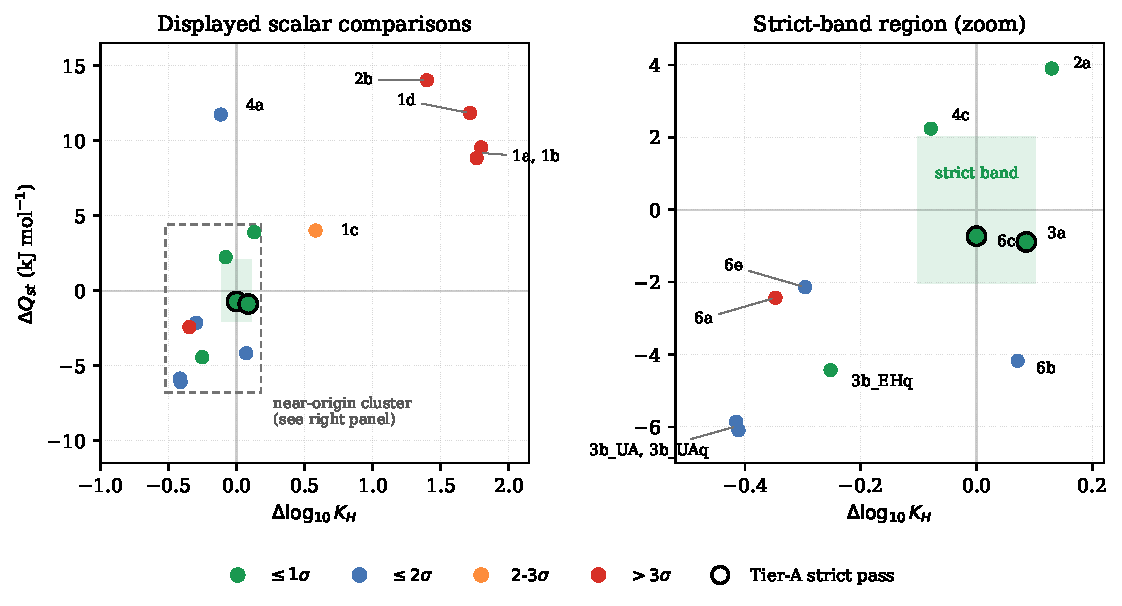
\includegraphics[width=\textwidth]{figures/fig2_strict_result.pdf}
\caption{Strict result. The scalar comparison rows of Table~\ref{tab:branch-disposition} in the deviation plane (\(\Delta\log_{10}K_H\), \(\Delta Q_{st}\)); the shaded box is the Tier-A strict band (\(\pm0.10\), \(\pm2.0\ \mathrm{kJ\,mol^{-1}}\)). Only 6c and 3a (black-edged) fall inside it --- the two-of-fifteen strict result. The right panel zooms on the near-origin region, where 2a, 4c, and 3b\_EHq sit just outside the band as Tier-B passes (3a sits inside, alongside 6c). The UiO-66 3b family is displayed in its three force-field variants; the headline denominator remains the fifteen-branch disposition described in Table~\ref{tab:branch-disposition} and Appendix~\ref{app:branch-table}. Deviations are read from the production runs --- 2a, 3a, and 4c from the v0.4.2 genuine-UFF / cross-engine rebuild; the 6c \(Q_{st}\) deviation is \(-0.73\ \mathrm{kJ\,mol^{-1}}\) (Dunne 1996 reference \(Q_{st}=15.7\ \mathrm{kJ\,mol^{-1}}\)). Branch 5b is method-blocked and is not plotted. Branch codes are internal locked-recipe identifiers; see the reader note in Section~\ref{sec:problem}.}
\label{fig:strict}
\end{figure}

\begin{figure}[tbp]
\centering
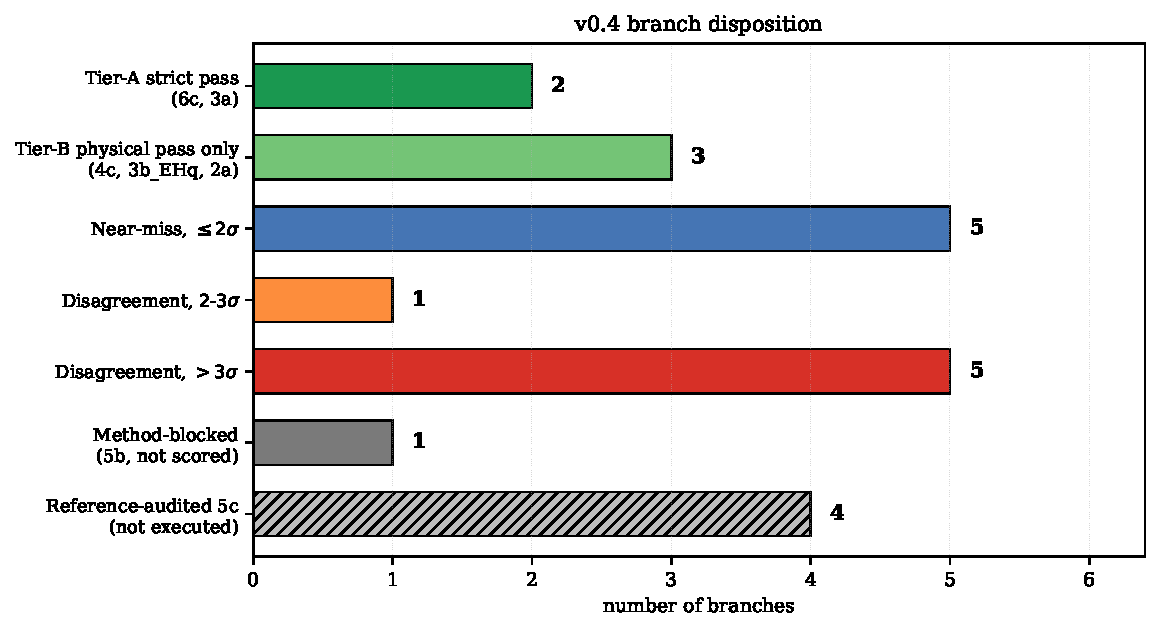
\includegraphics[width=0.80\textwidth]{figures/fig3_branch_disposition.pdf}
\caption{Branch disposition in mutually-exclusive outcome categories. The two Tier-A strict passes (6c, 3a) and the additional Tier-B physical passes (2a, 4c, 3b\_EHq) are the \(2/15\) and \(5/15\) headline; the remaining scalar rows are force-field disagreements and near-misses. The UiO-66 3b family is displayed in its three force-field variants, so the displayed scalar rows total sixteen but are counted as the locked fifteen-branch denominator (see Table~\ref{tab:branch-disposition} and Appendix~\ref{app:branch-table}). Branch 5b is method-blocked and not scalar-scored; the 5c cationic-zeolite targets are reference-audited and not executed. Counts are computed from the audited branch data. Branch codes are internal locked-recipe identifiers; see the reader note in Section~\ref{sec:problem}.}
\label{fig:disposition}
\end{figure}

Two of these branches are deliberate controls. Branch 6c is the simplest: all-silica MFI, argon, no charges, no flexible framework mechanism; it is a Tier-A strict pass cross-confirmed by the native estimator and RASPA3 to \(0.5\%\). Branch 4c is more demanding --- Si-CHA + CO\(_2\), Bai 2013 TraPPE-zeo parameters, electrostatics, and an analytical tail correction --- and is a cross-engine-audited charged control: the native estimator and RASPA3 agree to \(\sim\!9\%\) on \(K_H\) and \(\sim\!1\%\) on \(Q_{st}\), and the result sits inside the experimental window. Its strict-versus-Tier-B verdict is itself engine-dependent --- the \(Q_{st}\) deviation sits on the \(\pm2.0\) boundary (native \(+1.99\), inside; RASPA3 \(+2.24\), outside), so the same recipe is nominally strict on one engine and Tier-B on the other. We therefore report it as Tier-B, and note this as a worked example, on a charged system, of the verdict fragility this harness exists to expose.

The other two passes are audit-caught corrections, not controls. Branches 2a (HKUST-1 + CO\(_2\)) and 3a (UiO-66 + CO\(_2\)) were originally locked as a \(>3\sigma\) and a \(2\)--\(3\sigma\) force-field failure and read as ``UFF under-binds the open metal site.'' That reading was an artifact. The originally-locked recipe routed the MOF framework through a generator that hard-coded a zeolite/cation table and unconditionally stamped \texttt{source="UFF"} on framework atoms that were in fact the Harris-Yung CO\(_2\)-carbon (\(\epsilon = 28.1\) K vs genuine UFF \(52.8\)), TraPPE-zeo oxygen (\(53.0\) vs UFF \(30.2\)), and a wrong-\(\epsilon\) hydrogen --- only the metals were genuine UFF. Corrected to genuine UFF, the aromatic-linker dispersion compensates the genuinely weak UFF open-metal site and both MOFs reproduce experiment: 3a near-exactly (\(\Delta\log_{10}K_H = +0.086\), \(\Delta Q_{st} = -0.89\ \mathrm{kJ\,mol^{-1}}\); Tier-A strict), and 2a slightly over (\(K_H\) in the range \(8.3\)--\(10.8\ \mathrm{mol\,kg^{-1}\,bar^{-1}}\), reported as a range because of the open-Cu deep-well sampling tail; \(\Delta Q_{st} = +3.9\ \mathrm{kJ\,mol^{-1}}\); Tier-B). Both are reported from RASPA3 only: the native estimator cannot corroborate them because its charged-Ewald path shows a large, not-yet-root-caused discrepancy against RASPA3 on these MOF cells (Section~\ref{sec:controls}). This is a second worked example of the paper's own thesis --- a generator silently substituting parameters under a false label, caught by the harness --- parallel to the 6c silicon double-count. The originally-locked (buggy) deviations, \(\Delta\log_{10}K_H = -0.759\) (2a) and \(-0.802\) (3a), are retained in the case matrix as the documented superseded case.

A further Tier-B pass is different in kind again. Branch 3b\_EHq, UiO-66 + CO\(_2\) under the Maia 2023 explicit-hydrogen, Yang-charge variant, gives \(K_H = 2.87 \pm 0.094\ \mathrm{mol\,kg^{-1}\,bar^{-1}}\) and \(Q_{st} = 22.07 \pm 0.13\ \mathrm{kJ\,mol^{-1}}\), corresponding to \(\Delta \log_{10}K_H = -0.252\) and \(\Delta Q_{st} = -4.43\ \mathrm{kJ\,mol^{-1}}\). That is outside the strict band, but inside the physical-accuracy band defined for UiO-66. This is why it is not counted as a strict pass but is counted as a Tier-B physical pass.

Several branches are near-misses rather than clear successes. The united-atom UiO-66 variants, the MFI + CH\(_4\) Bai branch \cite{Hufton1993AIChE}, the Si-CHA Harris-Yung branch, and the MFI + Kr branch \cite{GoldenSircar1994JCIS} do not pass the strict gate. Some remain within the recorded two-sigma agreement class --- a diagnostic classification of the \(K_H\) log-space deviation, not a Tier-A pass criterion --- and several failures are dominated by \(Q_{st}\) rather than \(K_H\). These branches are useful because they show where a recipe is close enough to be scientifically informative but not close enough to be used as a strict validation point.

The strongest disagreements occur in the open-metal-site systems. Mg-MOF-74 + CO\(_2\) \cite{Mason2011EES,Britt2009PNAS,Queen2011JPCC,Wu2010JPCL,Simmons2011EES,Queen2014ChemSci} and HKUST-1 + CO\(_2\) \cite{Grajciar2011JPCC} expose a limitation of non-polarisable or simplified pairwise force fields at strong binding sites. Some branches over-bind and others under-bind, depending on the force-field family, but the common point is that the simple recipe does not transfer cleanly to the chemistry of the exposed metal site. The harness does not repair that failure; it names it.

The Na-Rho branch is a different case. Branch 5b is not scored as a scalar \(K_H/Q_{st}\) pass or fail. Rigid closed-state Widom samples a closed framework partition function, while the experimental adsorption observable involves a trapdoor opening process. The calculation and experiment are therefore not the same statistical-mechanical object. The site-geometry comparison can still be audited separately, but the scalar zero-coverage comparison is method-blocked.

The 5c cationic-zeolite family is also deliberately not treated as a hidden validation. Na-ZK-5, Zeolite 5A, Zeolite 13X, and Zeolite 4A have reference information recorded, but they require cation-containing structures and locked cation force-field and charge models before execution. Until those ingredients are supplied, they are reference-audited targets, not completed branches, and they do not validate Na-Rho.

The result is therefore smaller and more useful than a simple pass count. The atlas does not say that two passes make a general adsorption predictor. It says which recipes currently reproduce experiment, which recipes fail by force-field transferability, which are blocked by missing structures or incompatible references, and which are outside the rigid-Widom observable altogether. That is the value of the audit.

\FloatBarrier
   % Table 1 anchor lives here
% Section 7 --- What the failures mean
% normalisation needed (3b\_EHq already escaped; no smart-quotes).
% Discussion section: no numbers, no new citations.
\section{What the failures mean}\label{sec:failures}

The failures in Table~\ref{tab:branch-disposition} are not a single scientific event. They are different ways in which a calculated zero-coverage observable can lose contact with the experimental observable. That distinction is the main result of the negative branches. A failure caused by an inadequate force field, a failure caused by a wrong structure, and a failure caused by a different ensemble require different scientific responses (Figure~\ref{fig:taxonomy}).

\begin{figure}[tbp]
\centering
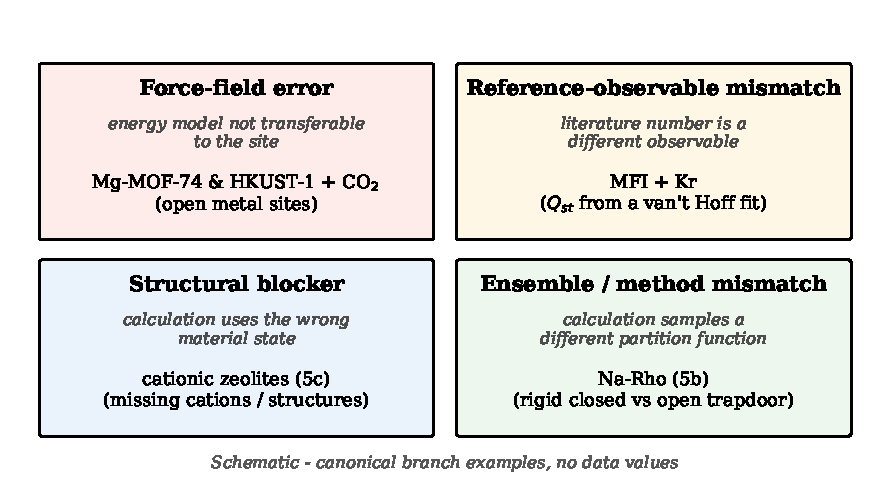
\includegraphics[width=0.86\textwidth]{figures/fig4_failure_taxonomy.pdf}
\caption{The four ways a calculated zero-coverage observable can lose contact with experiment, each with its canonical v0.4 branch example: force-field error (Mg-MOF-74 and HKUST-1 + CO\(_2\)), reference-observable mismatch (MFI + Kr, whose \(Q_{st}\) reference is a van't Hoff fit), structural blocker (cationic zeolites, 5c), and ensemble/method mismatch (Na-Rho, 5b). This figure is schematic and carries no numerical data.}
\label{fig:taxonomy}
\end{figure}

\FloatBarrier

The open-metal-site systems give the clearest force-field lesson. Mg-MOF-74 + CO\(_2\) and HKUST-1 + CO\(_2\) contain strongly binding metal environments. In such sites, carbon dioxide does not merely see a generic Lennard-Jones wall. It probes electrostatics, induction, short-range repulsion, dispersion, and local coordination chemistry. A non-polarisable or simplified pairwise force field can be reproducible and still give the wrong adsorption thermodynamics. That is what the atlas records: not that Widom insertion broke, but that the chosen energy model is not transferable enough for the site.

The direction of the error also matters. Some open-metal-site branches over-bind, while simpler UFF-type baselines under-bind. These are not contradictions. They show that different approximate energy models fail in different ways. A fitted cross-pair can put too much attraction into the binding site. A generic baseline can miss the same site. Both can be wrong for physically meaningful reasons. The audit prevents either result from being mistaken for a general statement about the material itself.

One caveat sharpens these force-field lessons. The comparison here is between the locked recipe and \emph{experiment}, not between the recipe and the originating paper's own simulated value, so an apparent over- or under-binding could in principle reflect a recipe difference or under-sampling rather than the energy model itself. Where the source recipe can be reproduced from the locked inputs, the atlas does reproduce the source's own simulated energetics: for HKUST-1 the modified Cu--O(CO\(_2\)) potential reproduces the paddle-wheel site interaction energy to within about two kilojoules per mole, and for UiO-66 the simulated heat of adsorption falls inside the band reported by the same study. For those branches the disagreement with experiment is therefore a genuine force-field-transferability result. For several Mg-MOF-74 recipes, however, the originating papers do not report a comparable simulated Henry constant or zero-coverage heat in the locked evidence, and in one case the atlas heat differs substantially from the source's own simulated value. For those branches the attribution to an intrinsic force-field limitation is reported here as unresolved pending a source-paper parity calculation, rather than as a proven force-field flaw. The open-metal-site Henry constant is also dominated by rare deep-well insertions --- in a representative audit, the hundred strongest of five thousand insertions account for roughly ninety percent of the Henry constant --- so production-count sampling is required and a low-count estimate is not converged.

The zeolite branches teach a different lesson. The clean all-silica MFI + Ar and Si-CHA + CO\(_2\) passes show that the harness can work when the structure, force field, and reference are aligned. They do not prove that all zeolite adsorption recipes are reliable. MFI + CH\(_4\), MFI + Kr, and the older Si-CHA + CO\(_2\) recipe still miss the strict gate. In several of these cases the problem is not simply the Henry constant. The heat of adsorption is the more sensitive axis, and its literature reference may itself come from a fitted or indirect observable.

The UiO-66 result is useful precisely because it is not a strict pass. The explicit-hydrogen, Yang-charge branch 3b\_EHq lies inside the physical-accuracy band but outside the strict regression band. That is the correct classification for a material whose reported adsorption is sensitive to synthesis, defects, and reference extraction. Calling it a strict validation point would overstate the result. Calling it a complete failure would throw away useful physical agreement. Tier-B exists to avoid both errors.

The cationic-zeolite cases are not force-field failures yet. They are incomplete recipes. Extra-framework cations are part of the material, not optional decoration. A pure-silica topology cannot stand in for Na-ZK-5, Zeolite 5A, Zeolite 13X, or Zeolite 4A when carbon dioxide adsorption is controlled by cation sites. Until the cation positions, charges, force-field parameters, and framework composition are locked, the calculation is not defined well enough to judge. Recording these systems as reference-audited targets is therefore more honest than forcing a pass or fail.

Na-Rho is still more restrictive. Its scalar branch is method-blocked because the rigid closed-state calculation and the trapdoor adsorption experiment do not sample the same configuration space. The problem is not merely that the force field needs tuning. The measured adsorption involves a framework-opening process, while the scalar Widom calculation samples a closed framework. The site-geometry evidence can be audited separately, but the scalar Henry constant and heat comparison cannot be converted into an ordinary validation test without changing the method.

This is why the small pass count is not a weakness of the audit. It is the audit doing its job. A less conservative workflow could report a number for every branch and then hide the reasons for disagreement in a table of residuals. widom-atlas instead separates reproducible agreement from force-field transferability failure, reference mismatch, structural incompleteness, and ensemble mismatch. The result is less flattering, but more useful.

The practical consequence is clear. For screening or machine-learning workflows, an adsorption number should not be consumed without its recipe and verdict. A strict-pass branch can be used as a calibrated validation point. A Tier-B branch can support a weaker physical-accuracy claim. A force-field-disagreement branch warns that the score is not reliable for the chemistry being tested. A method-blocked branch says that a different simulation observable is needed. The output of the atlas is therefore not just \(K_H\) or \(Q_{st}\). It is the reason those numbers should or should not be trusted.

% Section 8 --- What is missing
% normalisation needed (no smart-quotes, no underscores). Roadmap section;
% introduces 3 new citations: Witman2018JCTC, Becker2018JPCC, McCready2024JCTC.
\section{What is missing}\label{sec:missing}

The v0.4 result is deliberately incomplete. It proves that two locked recipes reproduce experiment within the strict band, and that three further recipes are physically credible within the wider Tier-B band. It does not prove that the atlas is finished. The value of the audit is that the remaining gaps are now named scientific tasks rather than hidden sources of error.

The first missing piece is a method for flexible or gate-opening adsorption. Na-Rho is the clearest example. A rigid closed-state Widom calculation cannot become a scalar validation of an experiment that involves a trapdoor opening process. Closing this gap requires a method that samples the relevant framework state or transition coordinate, not a different label on the same closed-state calculation. Possible routes include flat-histogram or transition-matrix approaches, or a mechanism-aware open-state adsorption calculation, but those would be new calculations rather than a reinterpretation of the v0.4 branch \cite{Witman2018JCTC}.

The second missing piece is a completed cationic-zeolite input set. The 5c family is already useful as a reference audit, but it is not yet an executed validation family. Na-ZK-5, Zeolite 5A, Zeolite 13X, and Zeolite 4A require cation-containing structures, cation positions, cation charges, and locked cation force-field parameters before the corresponding Widom recipes are defined. A topology-only or pure-silica framework would test the wrong material. The next step is therefore not simply to run more insertions, but to lock the correct structures and cation models.

The third missing piece is a better treatment of strong open-metal sites. The Mg-MOF-74 failures show that ordinary non-polarisable or simplified pairwise recipes are not enough for exposed metal centres (HKUST-1 under genuine UFF, by contrast, reaches the Tier-B band once its open-Cu site is supplemented by genuine aromatic-linker dispersion). One Mg-MOF-74 branch, 1c, also illustrates the silent-substitution defect class directly: its as-run framework Lennard-Jones parameters were plain UFF with a placeholder Mg \(\epsilon = 5.0\) K, not the ``reduced'' Becker values its label claimed --- a third audit-caught instance, retained here as a FAIL example rather than rebuilt. Polarisability, induction, and local coordination chemistry are plausible parts of the missing physics. A polarisable Mg-MOF-74 calculation is therefore a natural future target, but it is not a v0.4 result. Any such branch must be built as a new recipe, with its induced-dipole model, units, damping convention, and validation reference checked before it can affect a verdict \cite{Becker2018JPCC}.

The fourth missing piece is a quantitative consensus-reference layer. Some apparent failures depend as much on the reference observable as on the force field. A Henry constant from a low-pressure slope, a Toth fit, a Langmuir fit, a van't Hoff heat, and a calorimetric heat do not carry the same experimental meaning. Future versions should replace heuristic physical-accuracy bands with a systematic multi-source reference model where enough data exist. The goal is not to make the pass band wider, but to make the uncertainty in the reference observable explicit \cite{McCready2024JCTC}.

The fifth missing piece is a controlled route to machine-learned potentials. Machine-learned interatomic potentials may be useful where pairwise force fields miss the binding physics, especially at open metal sites. But they would change the recipe. A machine-learned potential is not a drop-in proof that Widom insertion is now predictive. It must be validated as its own energy model, with out-of-domain checks, hard-overlap handling, uncertainty diagnostics, and, where possible, comparison against electronic-structure reference calculations. No v0.4 strict pass used a machine-learned potential or GPU acceleration. Section~\ref{sec:v06} takes a first step on exactly this front: not a validated machine-learned adsorption branch, but a governance layer that characterises a machine-learned potential outside its training domain and, where the evidence supports it, screen-passes or withholds a verdict.

These missing pieces should not be confused with defects in the strict passes. The all-silica MFI + Ar (6c) and the genuine-UFF UiO-66 + CO\(_2\) (3a) results are valid for their locked recipes and references; the Si-CHA + CO\(_2\) branch (4c) is a cross-engine-checked Tier-B charged-zeolite control whose strict-versus-Tier-B verdict is engine-marginal. What is missing is the evidence needed to extend that reliability to harder classes of materials: flexible trapdoor zeolites, cationic zeolites, defective MOFs, and open-metal-site frameworks. The audit therefore points to a research programme rather than to a finished calculator.

These gaps fall into two groups that should not be confused. Section~\ref{sec:v06} reports one extension of exactly this governance logic that has already been carried out: cross-engine validation on CuspAI's kUPS engine and out-of-distribution governance of the machine-learned potential it ships. The remaining gaps named above --- flexible trapdoor methods, completed cationic-zeolite recipes, stronger open-metal-site models, and a quantitative consensus-reference layer --- are still future work, and each must be validated as a new locked recipe before it can affect any verdict.

The next version of the atlas should be judged by whether it closes these named gaps without weakening the standard of evidence. A new branch should not be promoted because it produces a convenient number. It should be promoted only when its structure, energy model, sampling method, reference observable, and verdict logic are explicit enough for another reader to reproduce and criticise. That is the standard v0.4 established, and it is the standard future work must preserve.

% Section --- v0.6 extension: cross-engine validation + MLIP governance on the kUPS stack.
% from a committed JSON in the version-controlled evidence base (see the standalone v0.6 report and CLAIMS.md).
\section{Cross-engine validation and machine-learned potentials}\label{sec:v06}

The harness above treats the simulation engine and the energy model as parts of the recipe. Two
questions follow. First, does the recipe transfer across engines: given the same locked recipe, does a
second, independently written estimator return the same observable? Second, the conclusion below
anticipates machine-learned potentials as new energy-model recipes; can the same governance distinguish
a trustworthy machine-learned adsorption number from an untrustworthy one? This section reports both,
retargeted onto CuspAI's JAX-native engine \emph{kUPS} and the machine-learning interatomic potential
(MLIP) it ships. Full numerical detail and the regeneration scripts are in the version-controlled evidence base.

\subsection{Cross-engine parity, and a silicon double-count caught by audit}\label{sec:v06-parity}

On the all-silica MFI + Ar positive control, the audit caught a subtler failure than a missing term: the
originally-locked 6c recipe \emph{double-counted silicon}, and agreed with its reference only as a fortuitous
cancellation of compounding errors. Talu--Myers' Ar--O cross-parameter (\(93.0\)~K) is the
Lorentz--Berthelot combination of argon with an oxygen-only \emph{effective} oxygen (\(72.2\)~K) that
already folds silicon's dispersion into oxygen --- Talu's model is oxygen-only by construction. The locked
recipe nonetheless added an explicit Ar--Si from an active framework silicon, counting silicon twice (a
factor \(1.8\) on \(K_H\)). That spurious term compensated three further errors --- an idealized rather
than the calibration (Olson) geometry, an under-converged \(12\)~\AA{} tail-off cutoff, and a reference
value mis-derived by \(\sim\!12\%\) --- which multiplied back to roughly the (wrong) reference. Removing
all four and running the coherent single-source recipe (pure Talu, oxygen-only) at a converged cutoff on
Talu's own geometry reproduces the \emph{corrected} reference (\(K_H = 0.200\)) exactly and cross-engine:
a native estimator gives \(0.200\) and RASPA3 \(0.199\) (parity \(0.5\%\)), the heat (\(14.97\) kJ/mol)
within \(0.7\) kJ/mol of the calorimetric value. The rebuild is deliberately not flattering on the heat:
at \(14.97\) kJ/mol it sits slightly farther from Dunne's \(15.7\) kJ/mol than the hybrid recipe's
\(\approx\!16.0\) kJ/mol, which is exactly what one expects if the original closeness was partly a
spurious-attraction cancellation rather than a coherent recipe. This is the paper's own thesis landing in its own
positive control --- a recipe assembled from incompatible silicon conventions yields a fortuitously-right
number, and only a governed single-source rebuild makes it honest --- in strict-band terms the hybrid lands in-band
against \emph{both} the mis-derived \(0.224\) (\(\Delta\log_{10}K_H = -0.034\)) and the corrected \(0.200\)
(\(+0.015\)), so the rebuild changes the
recipe's coherence, not the verdict (Table~\ref{tab:6c-cancellation}, Figure~\ref{fig:6c-cancellation}).
The reason the hybrid survived is quantitative: of the four errors, three are in the calculation
(silicon double-count \(\times1.80\), under-converged cutoff \(\times0.75\), non-calibration structure
\(\times0.77\)) and one is in the reference. The three computational errors compound to only
\(\times1.04\), so they very nearly cancel among themselves, and the fourth error moved the target to
meet them.

\paragraph{Structure sensitivity, and the limit of this control.} The converged single-source recipe is
not structure-independent. Evaluated on Talu's calibration (Olson) geometry \cite{Olson1981JPC} it gives
\(K_H = 0.200\ \mathrm{mol\,kg^{-1}\,bar^{-1}}\) and on the van Koningsveld geometry
\cite{vanKoningsveld1987ActaCrystB} \(0.205\), both
inside the strict window \([0.159, 0.252]\); on the IZA geometry the same recipe gives \(0.154\), which
is \emph{outside} that window (\(\Delta\log_{10}K_H = -0.114\)). Stated plainly: the clean recipe passes
strict on Talu's calibration geometry and fails strict on the IZA geometry, so the structure is a
verdict-affecting recipe element in its own right and not a detail. A second limit should be read with
this control: the Talu--Myers argon parameters were themselves fitted to silicalite adsorption data of
this kind, so three-figure agreement between this recipe and that reference is closer to a
self-consistency check on the calibration than to an independent validation of the energy model.

\begin{table}[tbp]
\centering\small
\caption{Branch 6c: the four-error cancellation in the originally-locked recipe, and the single-source
rebuild that removes each error in turn (reading down), reproducing the corrected reference on Talu's
calibration (Olson) geometry. The last rows show the structure sensitivity of the converged single-source
recipe.}\label{tab:6c-cancellation}
\begin{tabular}{@{}lcl@{}}
\toprule
recipe / setup & \(K_H\) (mol\,kg\(^{-1}\)\,bar\(^{-1}\)) & note \\
\midrule
locked 6c: hybrid, IZA, 12~\AA{} tail-off & 0.207 & in-band by a fortuitous cancellation (also passes 0.200) \\
\(\;\)remove the double-counted silicon & 0.115 & pure Talu, oxygen-only (IZA, 12~\AA{}) \\
\(\;\)+ converge the cutoff (24~\AA{} + tail) & 0.154 & numerical defect fixed (IZA) \\
\(\;\)+ Talu's calibration (Olson) geometry & \textbf{0.200} & native; RASPA3 \(0.199\), parity \(0.5\%\) \\
\midrule
corrected reference (Dunne 1996, \(K_H=B/kT\)) & \textbf{0.200} & strict window [0.159, 0.252] \\
structure sensitivity (single-source recipe) & 0.200 / 0.205 / 0.154 & Olson / van Koningsveld / IZA \\
\bottomrule
\end{tabular}
\end{table}

\begin{figure}[tbp]
\centering
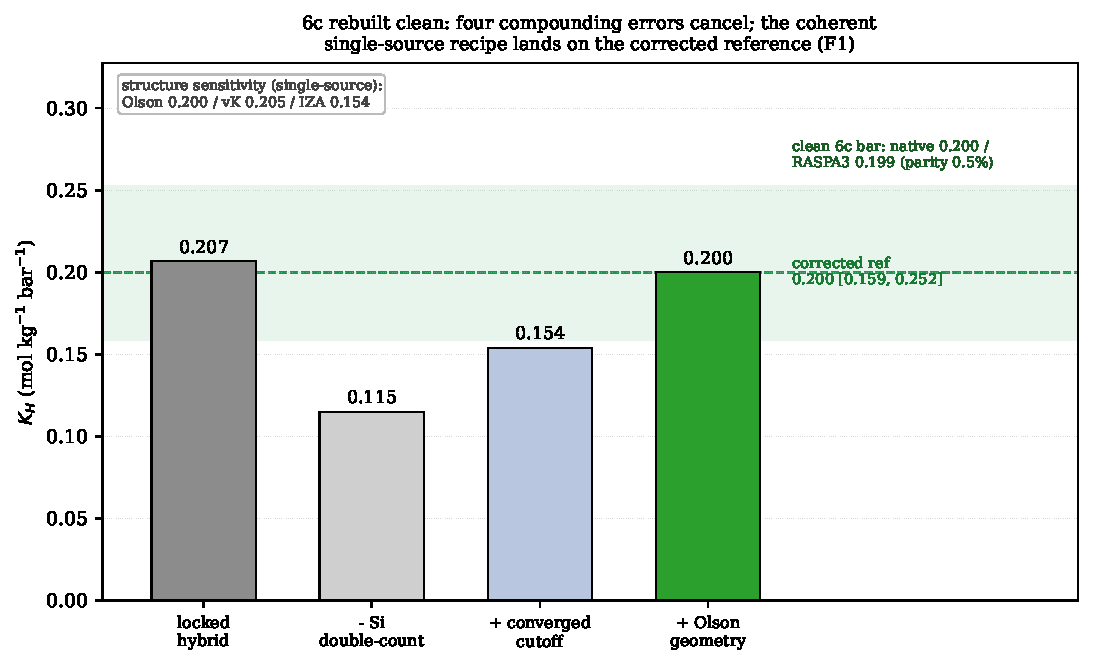
\includegraphics[width=0.78\textwidth]{figures/fp_6c_cancellation.pdf}
\caption{Finding F1 visualized: branch 6c rebuilt clean. The originally-locked hybrid recipe (\(0.207\))
agrees with the reference only as a fortuitous cancellation of four compounding errors; removing the silicon double-count,
converging the cutoff, and adopting Talu's calibration (Olson) geometry lands the coherent single-source
recipe on the corrected reference \(K_H = 0.200\), cross-engine (native \(0.200\), RASPA3 \(0.199\);
parity \(0.5\%\)). Values read from \texttt{cancellation\_6c.json}; the same chain is tabulated in
Table~\ref{tab:6c-cancellation}.}
\label{fig:6c-cancellation}
\end{figure}

\FloatBarrier

The same control provides, to our knowledge, the first published independent cross-engine validation of
the Widom test-particle estimator shipped in kUPS --- specifically the \texttt{kups.mcmc.widom} module,
as distinct from standalone Widom packages and from machine-learned-potential adsorption benchmarks such
as ODAC25~\cite{ODAC25}. The estimator is present in the engine source; a search of that source
found internal unit tests only, and the open issue tracker, inspected on 2026-06-12, carried one
unrelated feature request. On
two locked controls --- MFI + Ar without electrostatics, and Si-CHA + CO\(_2\) with framework charges and
Ewald summation --- kUPS reproduces the isosteric heat to \(0.22\) and \(0.01\) kJ/mol respectively; its
energies and its \(W=\exp(-\beta U)\) reduction are correct. The dominant \(K_H\) discrepancies trace to
named conventions: a \(+16\%\) gap on the Ar control root-causes to an LJ truncation convention (kUPS
truncates the potential at the cutoff where the reference shifts it; matching the convention reproduces
kUPS to \(+2.4\%\)), and the electrostatic control carries an additional tail-implementation difference.
One residual of order \(8\%\) remains, characterized as a normalization-flavoured, \(Q_{st}\)-invariant
scale and flagged open rather than hand-waved. Neither engine is wrong; the truncation convention is a
recipe element worth \(16\%\) on \(K_H\). The exponential sensitivity of \(K_H\) to a constant energy
offset, and the resulting need to lock the tail/truncation convention, are established
\cite{Jablonka2019,Dubbeldam2016}; what is new here is the cross-engine \emph{quantification} of the
effect, and the governed comparison is what makes it visible (Figure~\ref{fig:v06-parity}). The recipe these three engines share for this parity is the as-locked
hybrid reframed above as a silicon double-count; this does not weaken the validation, which tests whether
independent estimators agree on a \emph{common} recipe, not whether that recipe reproduces experiment. On the
convention-matched shifted recipe the native estimator and RASPA3 agree to \(1.1\%\) on \(K_H\); \(Q_{st}\) is
far less sensitive to the LJ shift convention, so kUPS stays within \(0.22\) kJ/mol of RASPA3 on the same
control even though its \(K_H\) carries the \(+16\%\) shifted-versus-truncated convention offset quantified above. The experimental-reproduction
correction --- silicon, structure, convention, reference --- lives entirely in the rebuilt control above;
the two findings are consistent.

\begin{figure}[tbp]
\centering
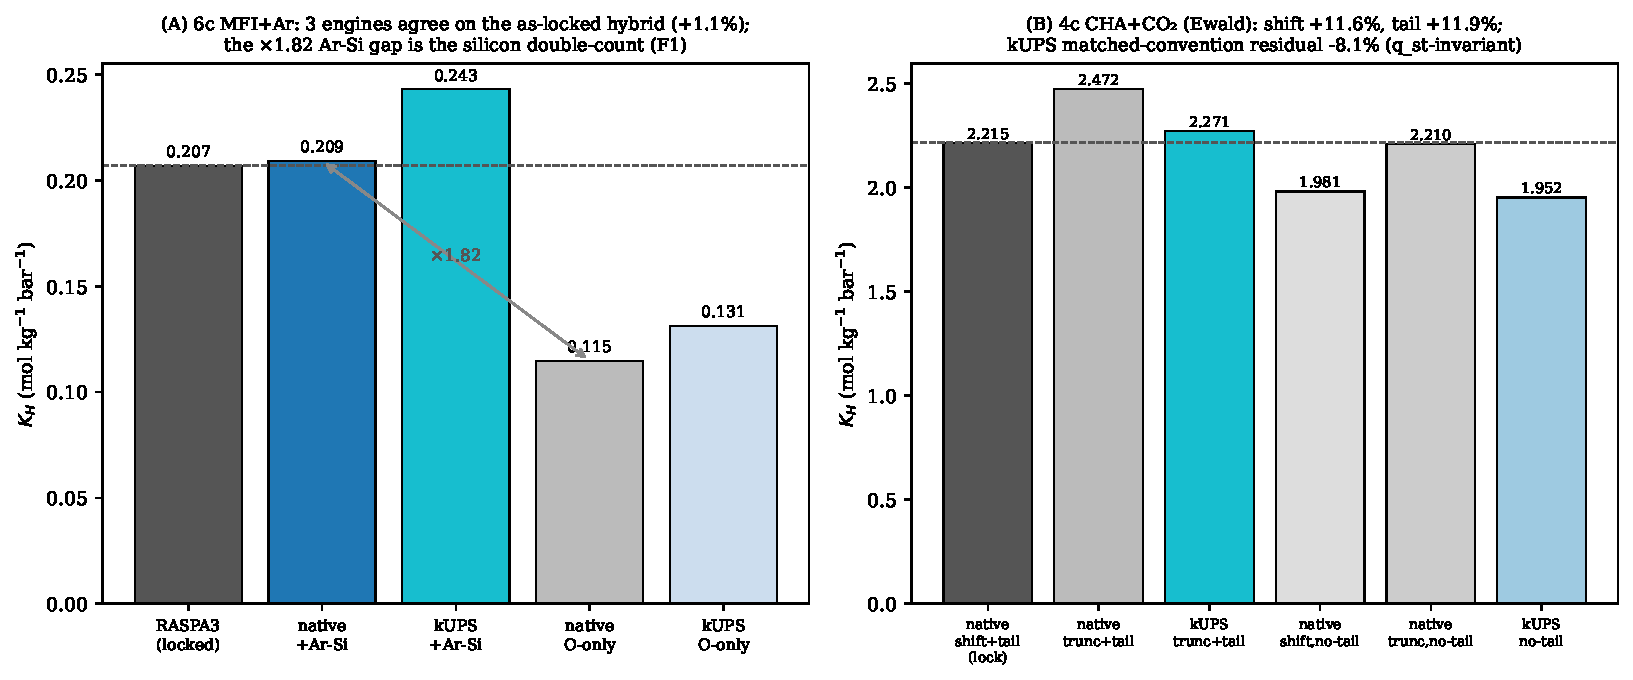
\includegraphics[width=\textwidth]{figures/fp_cross_engine_parity.pdf}
\caption{Cross-engine Widom parity. Left: on MFI + Ar, two independent estimators agree on the as-locked
hybrid recipe --- native + Ar--Si reproduces the locked RASPA3 reference --- and the factor-\(1.8\) gap to
the oxygen-only recipe is the silicon double-count of Finding~F1 quantified, not a legitimate missing
term. Right: the Si-CHA + CO\(_2\) (Ewald) convention matrix, isolating the LJ truncation shift and the
tail-implementation difference that account for the kUPS--reference offset.}
\label{fig:v06-parity}
\end{figure}

\FloatBarrier

\subsection{Machine-learned potentials as governed recipes}\label{sec:v06-mlip}

Treating an MLIP as one more energy-model recipe, we score Widom insertions of Ar into all-silica CHA
under four configurations, with a classical Lennard-Jones baseline scoring the same insertion geometries
so that every difference is the potential, not the sampling. The governance is a rule-based schema,
written before the results were seen and applied with one documented post-hoc correction (a spurious
weight clip, removed),
with two refusal classes: out-of-distribution over-binding (flagged insertions carry at least half the
Boltzmann weight) and absent-well under-binding (no physisorption minimum where one is established).
The second class is named for the observation rather than a mechanism: a flat positive plateau is
consistent with a missing dispersion term but equally with an unquantified out-of-distribution energy
offset, and the evidence here does not separate the two. The result
discriminates two distinct failure modes and, for one of them, certifies a governed screen-pass (Figure~\ref{fig:v06-triptych}). The 2023
MACE-MP-small potential hallucinates attractive energies \emph{inside} atomic overlaps --- its global
minimum, \(-19.3\) kJ/mol, lies at a hard overlap, and the flagged insertions carry \(99.5\%\) of the
weight; it is refused. The MACE-MPA-0 potential as shipped in CuspAI's \texttt{kUPS-mace-jax} export is
the opposite: repulsive everywhere (minimum \(+8.5\) kJ/mol), finding no physisorption well at all ---
consistent with the bare PBE signature of a missing dispersion term, although the plateau is flat with
distance and an out-of-distribution offset is not excluded; it too is refused. Pairing the \emph{same} weights with
the standard D3(BJ) dispersion correction recovers a physical well (minimum \(-5.0\) kJ/mol, shallower than the
\(-22\) kJ/mol classical baseline) at a non-overlap distance: it passes the out-of-distribution screen, accuracy
unassessed. Dispersion-correction on or off is therefore
a load-bearing recipe element, and an ungoverned pipeline silently differs on it. The kUPS in-engine JAX
export was verified energy-identical to the upstream reference implementation to a maximum relative
difference of \(2.1\times10^{-7}\), so the governance conclusions carry to the runtime path.

\paragraph{Audit correction to the overlap threshold.} The hard-overlap flag was applied at
\(0.80\,\sigma_{\min} = 2.762\)~\AA{}, built from \(\tfrac{1}{2}(3.500 + 3.405)\)~\AA{}. Those lengths
are not in the same convention: \(3.500\)~\AA{} is UFF's \(x_i\) for oxygen, which is \(r_{\min}\) and
not \(\sigma\) (\(\sigma = x_i/2^{1/6} = 3.118\)~\AA{}), while \(3.405\)~\AA{} is a Lennard-Jones
\(\sigma\) for argon. Re-derived self-consistently the threshold is \(2.626\)~\AA{}. Re-scoring the
committed per-insertion evidence changes no refuse or screen-pass verdict, but the UMA materials-head
flagged weight falls from \(0.998\) to \(0.000\), because its deepest insertion lies at \(2.646\)~\AA{}
--- inside the as-run overlap region and outside the corrected one. That refusal is therefore carried by
the energetic-anomaly gate, not the overlap gate, and the accurate description is that the potential is
erratic irrespective of overlap. A continuous \(U(r)\) scan along the line from the nearest framework
oxygen through that insertion confirms this: the anomaly is a smooth spurious basin reaching
\(-309.8\) kJ/mol at a host--guest separation of \(2.73\)~\AA{}, where the classical comparator on the
same trajectory is repulsive, and it reproduces on repeat to \(0.0005\) kJ/mol and shifts by a constant
\(0.195\) kJ/mol under a second reference configuration. The companion report carries the scan and the
full re-scoring. This is a \(\sigma \leftrightarrow r_{\min}\) slip of exactly the kind this paper is
about, caught by audit rather than by inspection.

\begin{figure}[tbp]
\centering
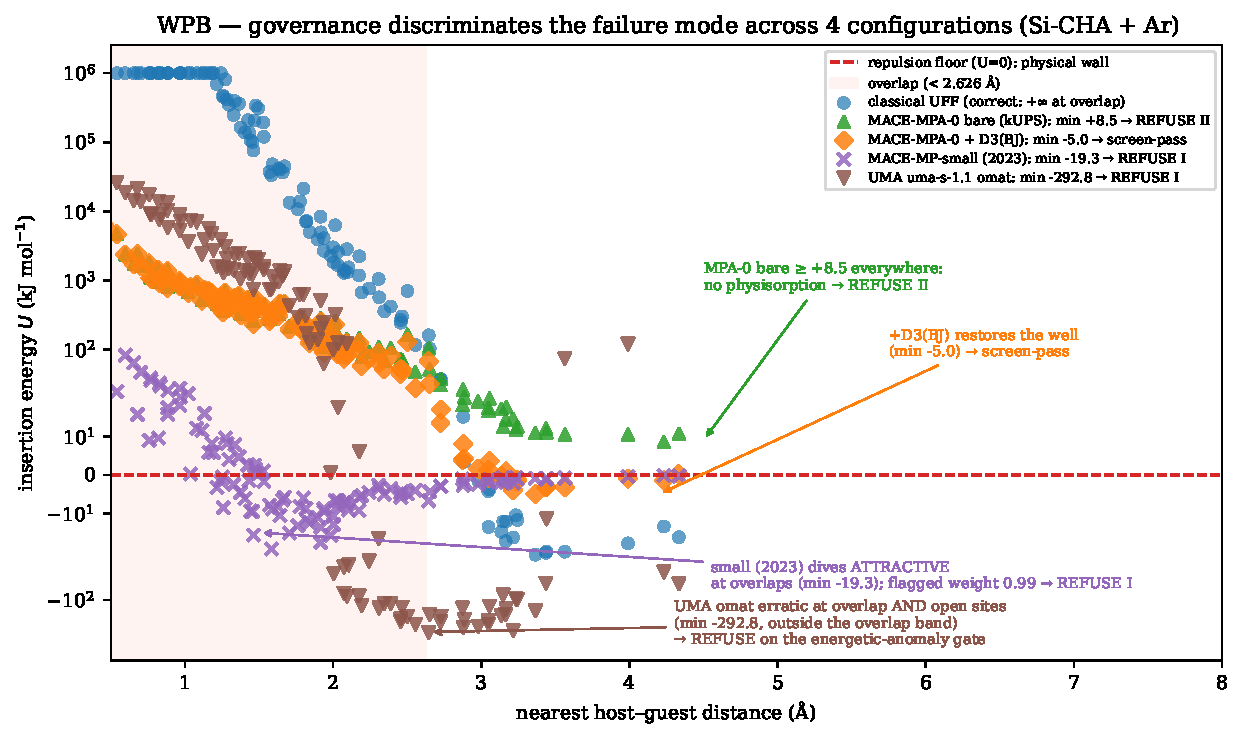
\includegraphics[width=\textwidth]{figures/f1_wpb_triptych.pdf}
\caption{Out-of-distribution governance discriminates the failure mode across four configurations
(Si-CHA + Ar). MACE-MP-small over-binds inside overlaps (refused); MACE-MPA-0 bare is repulsive
everywhere, finding no physisorption well (refused); the same weights with D3(BJ) recover a physical well
(screen-pass); the UMA materials head is erratic both inside and outside the overlap region and is
refused on the energetic-anomaly gate. The shaded band is the corrected \(2.626\)~\AA{} hard-overlap
threshold. Every label renders from a committed JSON.}
\label{fig:v06-triptych}
\end{figure}

\FloatBarrier

A multi-task foundation model sharpens the point that a verdict is only as good as the harness's right to
issue it. The UMA potential carries several level-of-theory heads; its choice is itself a recipe element.
Its materials head, used on Ar in silica, is erratic at close contact and is refused. Its direct-air-capture
head, used on Ar --- a noble gas outside its training distribution --- assigns energies that differ by
\(2.7\) kJ/mol between symmetry-equivalent open sites; the harness fails its own internal consistency
check and returns \emph{withheld}: no verdict, rather than a confident wrong one. The \emph{same}
direct-air-capture head, used on CO\(_2\) in the same framework --- CO\(_2\) is adsorbate-in-domain for this
head, though the all-silica CHA host lies outside the MOF host class used in its training --- is
self-consistent and finds a physical well (minimum \(-15.7\) kJ/mol, screen isosteric heat \(17.7\) kJ/mol
against a reference anchor of \(21.0\)): it passes the screen (Figure~\ref{fig:v06-uma}). The model passes
where its own documentation says it should, and is refused or withheld elsewhere. A screen-pass is not a
certificate of accuracy --- the runs are screens at \(N=60\)--\(120\) insertions, not converged
thermodynamics --- but it is the difference between a number that may be trusted and one that must not.

\begin{figure}[tbp]
\centering
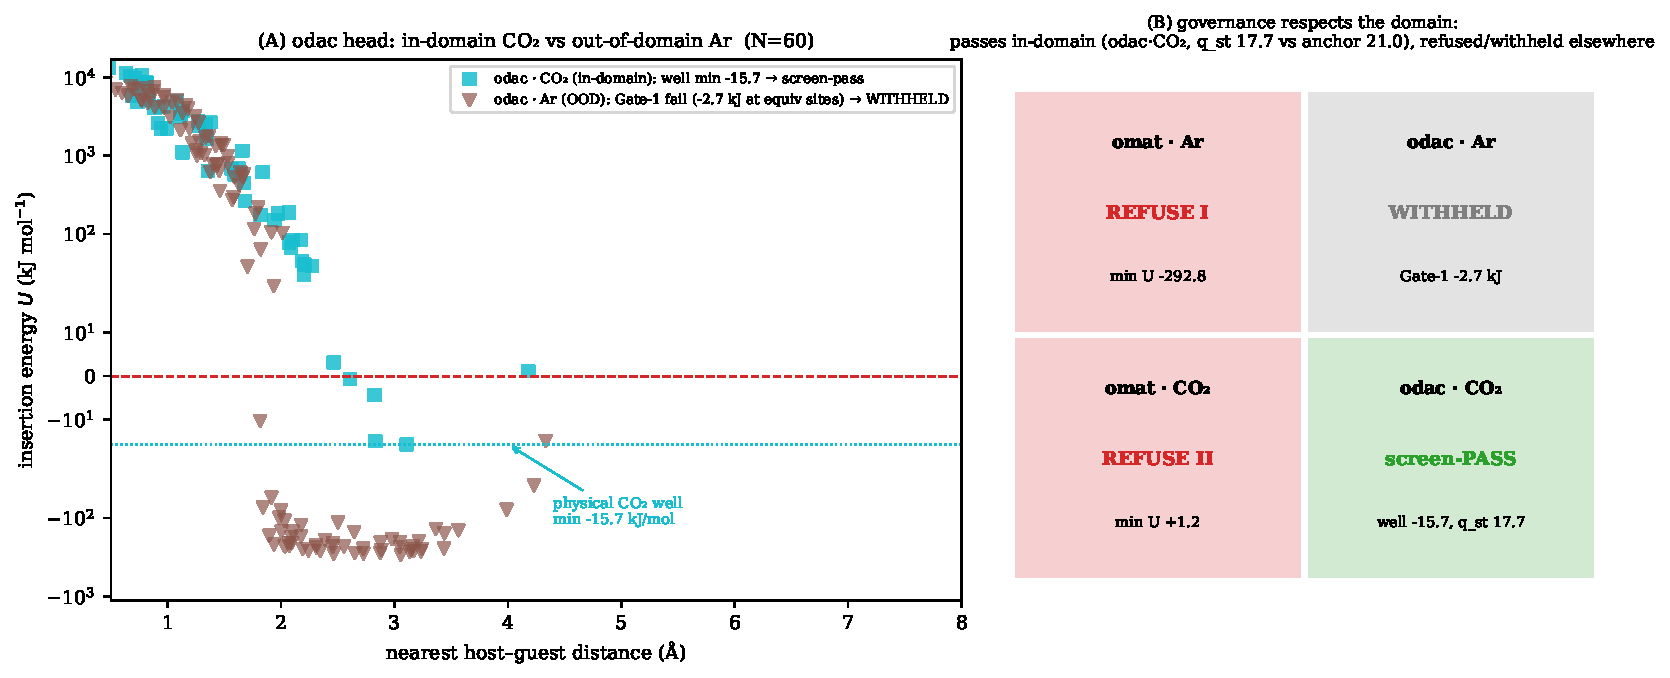
\includegraphics[width=\textwidth]{figures/f2_uma_domain.pdf}
\caption{Governance respects the model's domain. Left: the UMA direct-air-capture head screen-passes on
CO\(_2\) (adsorbate-in-domain; a physical well) and is withheld out-of-domain on Ar (internally inconsistent).
Right: the full task-by-system verdict matrix; the model passes where its adsorbate domain holds and is
refused or withheld elsewhere.}
\label{fig:v06-uma}
\end{figure}

\FloatBarrier

None of this changes the v0.4 verdict. It extends the same discipline to a second engine and to
machine-learned energy models, and it adds two recipe elements to the list that must be locked before a
Widom number is trustworthy: the engine's truncation convention, and the potential's domain of validity.
The point is unchanged. The trustworthy quantity is not the number; it is the number together with the
complete, locked recipe that produced it.

% Section 9 --- Conclusion
% normalisation needed (no smart-quotes, no underscores, no new citations).
% The final-sentence general-validation phrasing is the allowed negated form.
\section{Conclusion}\label{sec:conclusion}

widom-atlas began from a simple problem: a Widom insertion number is easy to compute, but hard to trust unless the calculation that produced it is completely specified. The Henry constant and zero-coverage isosteric heat are not merely outputs of an estimator. They are outputs of a structure, an atom typing, an energy model, a gas model, a mixing rule, an electrostatics convention, a backend, a sampling procedure, and a reference observable. The central claim of this paper is that this recipe must be treated as the scientific object.

The v0.4 audit gives a narrow result, presented as method-plus-audited-examples rather than a fifteen-branch certification. Two of fifteen verdict-affecting branches pass the strict criterion: the all-silica MFI + Ar positive control and the UiO-66 + CO\(_2\) branch under genuine UFF. Five of fifteen pass the Tier-B physical-accuracy criterion, adding HKUST-1 + CO\(_2\) under genuine UFF, the Si-CHA + CO\(_2\) Bai 2013 control, and the UiO-66 + CO\(_2\) Maia 2023 explicit-hydrogen variant. These results show that widom-atlas can reproduce experiment when the recipe and the reference are compatible --- and twice that conclusion survived only because the audit caught a defect first. The MFI + Ar control passed the strict band even as originally locked, but only as a fortuitous cancellation of four compounding errors; the cross-engine audit of Section~\ref{sec:v06} caught the silicon double-count and rebuilt the recipe clean (Finding~F1). The same audit caught a generator silently mislabelling the HKUST-1 and UiO-66 framework force fields, whose correction to genuine UFF moved both from apparent open-metal-site failures to physical-accuracy passes (one strict). They do not show that Widom insertion with standard force fields is generally predictive.

The negative branches are not failures of the same kind. The remaining open-metal-site systems --- the Mg-MOF-74 branches --- expose genuine force-field transferability limits. Some zeolite branches expose reference or heat-of-adsorption sensitivity. The cationic-zeolite targets remain incomplete recipes because the cation-containing structures and cation models are not yet locked. Na-Rho is method-blocked because a rigid closed-state Widom calculation and a trapdoor adsorption experiment are not the same statistical-mechanical observable. Treating all of these cases as ordinary failures would erase the physics that the audit is designed to reveal.

The useful product of widom-atlas is therefore not a larger table of adsorption numbers. It is a governed classification of those numbers. A branch can be a strict validation point, a weaker physical-accuracy point, a force-field disagreement, a reference-observable mismatch, a structural blocker, or an ensemble/method mismatch. This classification tells a screening workflow whether a score is a calibrated observable, a useful but weaker physical comparison, or a number that should not be trusted for the claimed purpose.

The present atlas is not finished. Flexible trapdoor zeolites require methods that sample the relevant framework states. Cationic zeolites require locked cation structures and cation force fields. Open-metal-site MOFs require energy models capable of the missing binding physics. Consensus references are needed where the literature observable itself is uncertain. Machine-learned potentials may become useful, but only as new energy-model recipes that must be validated on their own terms; Section~\ref{sec:v06} takes a first step in exactly that spirit, on the engine and the potential that CuspAI ships. None of these future tasks changes the v0.4 verdict.

The conclusion is therefore deliberately modest. widom-atlas is not scientifically validated as a general predictive adsorption tool. It is a reproducible way to decide whether a particular Widom adsorption number is a trustworthy zero-coverage observable or merely the output of an untested recipe. That distinction is the result.


% ====================== APPENDICES (A--E) ======================
\appendix
% Appendix A --- Estimator details. Populated 2026-06-09 from the main-text
% beyond the main text.
\section{Estimator details}\label{app:estimator}

This appendix records the estimator and unit details behind the equations of Section~\ref{sec:observable}. It introduces no physics beyond the main text.

For a guest in a rigid host at temperature \(T\), widom-atlas estimates the zero-coverage Henry constant by Widom insertion as
\[
K_H = \frac{V}{M\,k_B\,T\,N_A}\,\bigl\langle \exp(-\beta U)\bigr\rangle,
\]
and the zero-coverage isosteric heat as the Boltzmann-weighted mean insertion energy plus the ideal-gas thermal term,
\[
Q_{st} = -\,\frac{\bigl\langle U\,\exp(-\beta U)\bigr\rangle}{\bigl\langle \exp(-\beta U)\bigr\rangle} + RT.
\]
Here \(U\) is the host--guest interaction energy of a single inserted, non-perturbing test molecule; \(\beta = 1/(k_B T)\), with \(k_B\) the Boltzmann constant; \(V\) and \(M\) are the simulation-cell volume and mass; \(N_A\) is Avogadro's constant; \(R\) is the molar gas constant; \(T\) is the temperature; and \(\langle\,\cdot\,\rangle\) denotes the average over uniformly sampled insertion positions and orientations in the rigid host.

The first estimator is reported in \(\mathrm{mol\,kg^{-1}\,bar^{-1}}\) and the second in \(\mathrm{kJ\,mol^{-1}}\). The conversion from the raw simulation quantities to these reported units is part of the locked recipe, not a formatting step.

These estimators are exact only for the specified rigid host structure and the specified energy model, in the dilute-gas limit. They are not exact for the material unless the locked structure and energy model are the correct ones for the experiment being compared against; that is the distinction developed in the main text.

A test insertion that overlaps a host atom produces a large positive \(U\), so its Boltzmann weight \(\exp(-\beta U)\) is negligible. Such severe overlaps therefore contribute essentially nothing to either average, which is why a short-range hard core does not bias the estimators.

Sampling uncertainty is estimated from independent random-number-generator seeds: each branch is run with several seeds, and the reported \(\pm\) values are the seed-to-seed standard deviations of \(K_H\) and \(Q_{st}\). The recorded per-branch seed and insertion counts are listed in Appendix~\ref{app:compute}.

% Appendix B --- Numerical lock and reproducibility. Populated 2026-06-09 from
% the scientific status lock, src/.../thresholds.py, and the production verdicts.
% No values recomputed; no unverified software-version claims.
\section{Numerical lock and reproducibility}\label{app:lock}

This appendix records the numerical identity of the v0.4 result. All values are read from the locked case matrix, the scientific status lock, and the production verdict JSONs; none is recomputed here.

\paragraph{Locked case matrix.} The v0.4 case matrix is pinned by the SHA-256 digest
\begin{center}\small\ttfamily
CASE\_MATRIX\_SHA256 =\\
b0571780a4794be0fabb2a7d47a093fcb8dab07c4355467bb2fabe1a6a085664\\
8c943c3890847dfe6d98f684211d449e
\end{center}
A locked-input loader verifies this digest before any consumer reads the matrix.

\paragraph{Strict acceptance thresholds.} The Tier-A strict (regression) band is \(\pm 0.10\) in \(\Delta\log_{10} K_H\) and \(\pm 2.0\ \mathrm{kJ\,mol^{-1}}\) in \(\Delta Q_{st}\). It is a tight reproducibility gate, deliberately tighter than experimental scatter, and is not itself a physical-accuracy claim. Acceptance is \emph{inclusive}: a branch passes when \(|\Delta\log_{10}K_H| \le 0.10\) and \(|\Delta Q_{st}| \le 2.0\ \mathrm{kJ\,mol^{-1}}\). The decision is taken on the three-seed point estimate; the seed-to-seed standard deviation (for example \(\pm 0.33\ \mathrm{kJ\,mol^{-1}}\) on the 4c heat) is reported as a reproducibility indicator and is not folded into the pass/fail logic. Branch 4c sits exactly on the heat boundary, and which side it lands on is engine-dependent: on the native estimator \(\Delta Q_{st} = +1.99\ \mathrm{kJ\,mol^{-1}}\) (inside), on RASPA3 \(+2.24\) (outside). The same recipe is therefore nominally strict on one engine and Tier-B on the other; we report 4c as Tier-B (the cross-engine \(K_H\) agreement is \(\sim\!9\%\) and the result is inside the experimental window).

\paragraph{Headline disposition.} Two of fifteen verdict-affecting branches pass the strict criterion: 6c (all-silica MFI + Ar) and 3a (UiO-66 + CO\textsubscript{2} under genuine UFF). Five of fifteen pass the Tier-B physical-accuracy criterion: 6c, 3a, 2a (HKUST-1 + CO\textsubscript{2}, genuine UFF), 4c (Si-CHA + CO\textsubscript{2} under the Bai 2013 TraPPE-zeo recipe), and 3b\_EHq (UiO-66 + CO\textsubscript{2}, explicit-hydrogen Yang-charge Maia 2023 variant). The 2a/3a passes are the v0.4.2 genuine-UFF rebuild that corrected a generator mislabel (see the audit result); their superseded as-locked deviations are retained in the case matrix.

\paragraph{Branches that are not scalar-scored.} Branch 5b (Na-Rho + CO\textsubscript{2}) is method-blocked: a rigid closed-state Widom calculation and the open-state trapdoor adsorption experiment are different statistical-mechanical observables, so the scalar \(K_H\)/\(Q_{st}\) comparison is not scored as a pass or a fail. The 5c cationic-zeolite targets (Na-ZK-5, Zeolite 5A, Zeolite 13X, Zeolite 4A) are reference-audited only: their experimental references are recorded, but the cation-containing structures and cation force-field and charge models are not locked, so they are not executed validation branches and do not validate 5b.

\paragraph{Scope of the v0.4 claim.} On this evidence, widom-atlas is not scientifically validated as a general predictive adsorption tool. No v0.4 strict pass used a machine-learned interatomic potential or GPU acceleration.

\paragraph{Backend-agreement controls (as recorded).} The native Lennard-Jones evaluator agrees with RASPA3 to within one percent on the all-silica MFI + Ar and MFI + CH\textsubscript{4} recipes. On the Si-CHA + CO\textsubscript{2} charged-framework control (4c) the native Ewald estimator and RASPA3 agree to \(\sim\!9\%\) on \(K_H\) and \(\sim\!1\%\) on \(Q_{st}\). On HKUST-1, by contrast, the native charged-Ewald path shows a large empirical discrepancy against RASPA3 --- about a factor of four on the identical recipe. A suspected non-orthogonal minimum-image explanation was tested after the audit; at the actual supercells and cutoffs of the published runs, a brute-force image check found no within-cutoff mis-imaged pairs for HKUST-1, Si-CHA, or MFI, so the root cause is \emph{not} established. The native charged-MOF results are therefore treated as non-verdict-supporting; the MOF branches are reported from RASPA3 (2a, 3a) or RASPA2 (1a). The 4c result is retained because it is directly cross-engine checked, not because of any orthogonality assumption. The Mg-MOF-74 + CO\textsubscript{2} Buckingham recipe was run on RASPA2; the native Buckingham path is not independently cross-validated on this MOF. The MOF branches presented only as audited examples (1b, 1c, 1d, 2b, 3b) inherit this limitation. No headline result depends on the native charged-MOF path. The specific backend build versions are recorded in the locked case matrix and are not restated here.

% Appendix C --- Full branch table. Populated 2026-06-09. The provenance table
% below is generated from the SAME source as the main-text Table 1: the
% production verdict JSONs (evidence/v04_two_tier/verdicts/*.json, plus
% v04_4c_bai_2013 and v04_6e_bai_2013). 5b scalar columns are em-dashes; 5c is
% not listed as an executed validation row.
\section{Full branch table}\label{app:branch-table}

Table~\ref{tab:branch-disposition} in the main text is the compact branch-disposition table. This appendix records the per-branch provenance behind it.

\paragraph{The fifteen-branch denominator.} The headline strict-pass denominator is fifteen verdict-affecting scalar branches. The UiO-66 3b case is run in three force-field variants (united-atom; united-atom + charges; explicit-hydrogen + charges). These variants are shown separately below for transparency, but they are counted according to the locked v0.4 disposition rather than as three independent denominator slots. Branch 5b is method-blocked and is not scalar-scored, so it does not enter the scalar denominator. The 5c cationic-zeolite targets are reference-audited only and are not executed validation branches; they are recorded in Appendix~\ref{app:lock} and are deliberately not listed as rows here, so that the table cannot be read as if they validated Na-Rho. The displayed scalar comparison rows are therefore not the same object as the locked headline denominator: the fifteen locked verdict-affecting branches expand to sixteen displayed scalar rows (the UiO-66 3b family in its three force-field variants), while branch 5b is method-blocked and the four 5c targets are reference-audited, both outside the scalar denominator.

\paragraph{Provenance table.} Table~\ref{tab:appendix-c} lists, for each scalar branch, the per-axis deviations, the Tier-A and Tier-B verdicts, the recorded agreement class, and the production verdict directory. The deviation values are those used for Table~\ref{tab:branch-disposition}, read from the verdict JSONs. For the method-blocked branch 5b the scalar columns are blank.

{\scriptsize
\setlength{\tabcolsep}{3pt}
\renewcommand{\arraystretch}{1.15}
\begin{longtable}{@{}l>{\raggedright\arraybackslash}p{0.12\textwidth}rrcccl@{}}
\caption{Per-branch provenance behind Table~\ref{tab:branch-disposition}. Tier A is the strict regression gate ($\pm0.10$ / $\pm2.0$); Tier B is the per-system physical-accuracy band; Class is the recorded agreement class (a diagnostic, not a Tier-A criterion); Source is the production verdict directory. Branch 5b is method-blocked, so its scalar columns are blank; the reference-audited 5c targets are not listed.}\label{tab:appendix-c}\\
\toprule
Br. & System & $\Delta\log_{10}K_H$ & $\Delta Q_{st}$ & Tier A & Tier B & Class & Source \\
\midrule
\endfirsthead
\multicolumn{8}{@{}l}{\footnotesize\emph{Table~\ref{tab:appendix-c}, continued}}\\
\toprule
Br. & System & $\Delta\log_{10}K_H$ & $\Delta Q_{st}$ & Tier A & Tier B & Class & Source \\
\midrule
\endhead
\midrule
\multicolumn{8}{@{}r}{\footnotesize\emph{continued on next page}}\\
\endfoot
\bottomrule
\endlastfoot
6c & MFI + Ar & $0.000$ & $-0.73$ & PASS & PASS & $\le 1\sigma$ & v04\_6c\_olson\_clean \\
4c & Si-CHA + CO\textsubscript{2} & $-0.079$ & $+2.24$ & FAIL & PASS & $\le 1\sigma$ & v04\_4c (RASPA3 xcheck) \\
3b\_EHq & UiO-66 + CO\textsubscript{2} & $-0.252$ & $-4.43$ & FAIL & PASS & $\le 1\sigma$ & v04\_two\_tier \\
3b\_UA & UiO-66 + CO\textsubscript{2} & $-0.411$ & $-6.09$ & FAIL & FAIL & $\le 2\sigma$ & v04\_two\_tier \\
3b\_UAq & UiO-66 + CO\textsubscript{2} & $-0.415$ & $-5.86$ & FAIL & FAIL & $\le 2\sigma$ & v04\_two\_tier \\
4a & Si-CHA + CO\textsubscript{2} & $-0.116$ & $+11.74$ & FAIL & FAIL & $\le 2\sigma$ & v04\_two\_tier \\
6b & MFI + Kr & $+0.071$ & $-4.17$ & FAIL & FAIL & $\le 2\sigma$ & v04\_two\_tier \\
6e & MFI + CH\textsubscript{4} & $-0.296$ & $-2.14$ & FAIL & FAIL & $\le 2\sigma$ & v04\_6e\_bai\_2013 \\
1c & Mg-MOF-74 + CO\textsubscript{2} & $+0.581$ & $+4.01$ & FAIL & FAIL & $2$--$3\sigma$ & v04\_two\_tier \\
3a & UiO-66 + CO\textsubscript{2} & $+0.086$ & $-0.89$ & PASS & PASS & $\le 1\sigma$ & v0.4.2 rebuild \\
1a & Mg-MOF-74 + CO\textsubscript{2} & $+1.765$ & $+8.83$ & FAIL & FAIL & $>3\sigma$ & v04\_two\_tier \\
1b & Mg-MOF-74 + CO\textsubscript{2} & $+1.799$ & $+9.55$ & FAIL & FAIL & $>3\sigma$ & v04\_two\_tier \\
1d & Mg-MOF-74 + CO\textsubscript{2} & $+1.716$ & $+11.84$ & FAIL & FAIL & $>3\sigma$ & v04\_two\_tier \\
2a & HKUST-1 + CO\textsubscript{2} & $+0.13$ & $+3.9$ & FAIL & PASS & $\le 1\sigma$ & v0.4.2 rebuild \\
2b & HKUST-1 + CO\textsubscript{2} & $+1.400$ & $+14.03$ & FAIL & FAIL & $>3\sigma$ & v04\_two\_tier \\
6a & MFI + CH\textsubscript{4} & $-0.347$ & $-2.43$ & FAIL & FAIL & $>3\sigma$ & v04\_two\_tier \\
\addlinespace[2pt]
5b & Na-Rho + CO\textsubscript{2} & --- & --- & --- & --- & --- & lock \\
\end{longtable}
}

Branch 5b is shown with blank scalar columns because it is method-blocked (an ensemble mismatch between the rigid closed-state calculation and the open-state experiment) and is not scored on a scalar \(K_H\)/\(Q_{st}\) axis.

\paragraph{On the agreement class.} The agreement class is a diagnostic classification recorded by the audit pipeline: it is the agreement of the \(K_H\) deviation in log space, computed as a z-score \(\Delta\log_{10}K_H / \sigma\) with an assumed experimental scatter \(\sigma = 0.05\) in \(\log_{10}K_H\). It does not encode \(Q_{st}\). It is not used as a Tier-A pass criterion and should not be read as a posterior probability unless the corresponding uncertainty model is inspected.

\FloatBarrier

% Appendix D --- Computational resources. Populated 2026-06-09 from the
% production verdicts (recorded seed/insertion counts) and the data pack.
% No hardware bragging; no implication that GPU was used for v0.4.
\section{Computational resources}\label{app:compute}

The v0.4 strict results are CPU-reproducible and are not GPU-dependent. No v0.4 strict pass used a machine-learned interatomic potential or GPU acceleration.

The two strict-pass branches are 6c (MFI + Ar) and 3a (UiO-66 + CO\textsubscript{2} under genuine UFF). Their recorded sampling is: 6c with three independent seeds of \(200{,}000\) Widom insertions on the native estimator and a RASPA3 cross-check (evidence \texttt{evidence/v04\_6c\_olson\_clean}); and 3a with twelve independent RASPA3 seeds of \(400{,}000\) cycles each at \(298.15\) and \(323.15\) K --- the v0.4.2 genuine-UFF rebuild (evidence \texttt{evidence/v04\_3a\_genuine\_uff}). The Si-CHA + CO\textsubscript{2} charged control (4c, Tier-B) was run with three independent seeds of \(60{,}000\) insertions on the native estimator and cross-checked on RASPA3 (evidence \texttt{evidence/v04\_4c\_bai\_2013}). These are the seed and insertion counts recorded in the committed evidence. Per-branch wall-time figures beyond these counts are not part of the locked v0.4 record and are therefore not stated here.

Heavier future work --- machine-learned interatomic potentials, polarisable energy models, or broader branch sweeps --- may benefit from GPU acceleration or larger workstations. Such work is not part of the v0.4 verdict, and the v0.4 strict passes reported here do not depend on it.

% Appendix E --- v0.5 non-load-bearing notes. Populated 2026-06-09. Keeps v0.5
% clearly future-work and non-load-bearing; does not make any v0.5 finding
% load-bearing on the v0.4 verdict.
\section{v0.5: non-load-bearing extension notes}\label{app:v05}

\textbf{Version map.} v0.4 is the locked classical audit matrix; v0.4.2 is the corrected rebuild and provenance layer for the audited examples (the genuine-UFF 2a and 3a, the cross-engine-checked 4c, and the clean 6c rebuild); v0.5 contains non-load-bearing extension notes only (this appendix); v0.6 is the kUPS and MLIP governance companion, summarised in Section~\ref{sec:v06}. Only the stated locked branches and committed evidence affect the v0.4/v0.4.2 verdicts.

The work described in this appendix is future work, and it does not change the v0.4 verdict. Any v0.5 feature or review branches that exist are non-load-bearing: none of them is used in, or alters, the v0.4 result reported in the main text.

The future extensions under consideration are: a polarisable treatment of Mg-MOF-74 + CO\textsubscript{2}; a quantitative multi-source consensus-reference layer; completion of cation-containing zeolite structures and cation models; and machine-learned-potential or ASE-calculator routes. Each is a future extension only, and each would have to be validated as a new recipe on its own terms before it could affect any verdict.

None of these extensions changes the v0.4 disposition. None changes the strict-pass result of two of fifteen branches. None changes the Tier-B physical-accuracy result of five of fifteen branches. None converts the method-blocked Na-Rho (5b) scalar comparison into a pass or a fail. And none makes the reference-audited 5c cationic-zeolite targets a completed validation family.


\section*{Code and data availability}

The public release repository for widom-atlas is \url{https://github.com/wseltd/widom-atlas-release}. It contains the manuscript source, the locked case matrix, the figure scripts, and the curated committed evidence JSON used for the reported values. The internal branch identifiers in the paper are retained to make the text traceable to that repository evidence.

% ============ ACKNOWLEDGEMENTS (unnumbered; before References) ============
% Author-supplied text, added verbatim 2026-06-09 per author instruction.
\section*{Acknowledgements}

The author thanks The London Library for the quiet of its reading rooms, where much of this manuscript was thought through and revised. He also thanks the Library for the use of its printers during drafting; they were asked to produce more intermediate versions than any sensible machine should have had to tolerate.

% ====================== REFERENCES ======================
% Backstop: flush every pending float and start a fresh page BEFORE the
% bibliography, so no result table can ever strand after the references.
\FloatBarrier
\clearpage
\bibliographystyle{unsrt}
\bibliography{references}

\end{document}
